%----------------------------------------------------------------------------------------
%       PACKAGES AND OTHER DOCUMENT CONFIGURATIONS
%----------------------------------------------------------------------------------------

\documentclass[
        % a4paper, % Page size
        fontsize=10pt, % Base font size
        twoside=true, % Use different layouts for even and odd pages (in particular, if twoside=true, the margin column will be always on the outside)
        %open=any, % If twoside=true, uncomment this to force new chapters to start on any page, not only on right (odd) pages
        %chapterentrydots=true, % Uncomment to output dots from the chapter name to the page number in the table of contents
        numbers=noenddot, % Comment to output dots after chapter numbers; the most common values for this option are: enddot, noenddot and auto (see the KOMAScript documentation for an in-depth explanation)
]{kaobook}

\usepackage[utf8]{inputenc}
\usepackage{CJKutf8} % Japanese
\usepackage{amsmath}
\usepackage{amssymb}
\usepackage{amsfonts}
\usepackage{stmaryrd}
\usepackage{array}
\usepackage{graphicx}
\usepackage{hyperref}
\usepackage{listings}
\usepackage{makeidx}
\usepackage[all]{xypic}

\usepackage[english]{babel} % Load characters and hyphenation
\usepackage[english=american]{csquotes}  % English quotes

% Load the bibliography package
\usepackage[backend=bibtex,sorting=nyt]{kaobiblio}
\addbibresource{notes.bib} % Bibliography file
\addbibresource{cca.bib} % Bibliography file
\addbibresource{realizability.bib} % Bibliography file

% Load mathematical packages for theorems and related environments
\usepackage[
  definitionbackground=green!10!white,
  theorembackground=blue!10!white,
  propositionbackground=Goldenrod!20!white,
  lemmabackground=Goldenrod!20!white,
  corollarybackground=Goldenrod!20!white,
  framed=true]{kaotheorems}

% Load the package for hyperreferences
\usepackage{kaorefs}

\crefname{embeddingTheorem}{Embedding Theorem}{Embedding Theorems}
\crefname{extensionTheorem}{Extension Theorem}{Extension Theorems}


%\graphicspath{{images/}} % Paths in which to look for images

\makeindex[columns=3, title=Alphabetical Index, intoc] % Make LaTeX produce the files required to compile the index

%\makeglossaries % Make LaTeX produce the files required to compile the glossary
%\input{glossary.tex} % Include the glossary definitions

% \makenomenclature % Make LaTeX produce the files required to compile the nomenclature

% Reset sidenote counter at chapters
%\counterwithin*{sidenote}{chapter}

%%% Settings for listings
\lstset{style=kaolstplain}
\lstset{xleftmargin=2em}

%\newenvironment{proof}{\medskip\noindent\emph{Proof.}}{\hfill$\Box$\medskip}

\newcommand{\defemph}[1]{\emph{\textbf{#1}}}

%%% Blackboard bold letters
\newcommand{\NN}{\mathbb{N}}
\newcommand{\NNx}{{\NN^{+}}}
\newcommand{\ZZ}{\mathbb{Z}}
\newcommand{\QQ}{\mathbb{Q}}
\newcommand{\RR}{\mathbb{R}}
\newcommand{\CC}{\mathbb{C}}

%%% PCAs
\renewcommand{\AA}{\mathbb{A}}
\newcommand{\subAA}{\mathbb{A}'}
\newcommand{\EE}{{\mathbb{E}}}
\newcommand{\subEE}{{\mathbb{E}'}}
\newcommand{\FF}{{\mathbb{F}}}
\newcommand{\subFF}{{\mathbb{F}'}}
\newcommand{\GG}{{\mathbb{G}}}
\newcommand{\subGG}{{\mathbb{G}'}}

\newcommand{\klone}{\mathbb{K}_1}
\newcommand{\UU}{\mathbb{U}}

\newcommand{\CL}{\mathbb{CL}}

%%% Applicative morphisms
\newcommand{\ff}[1]{\widehat{#1}}  % functor induced by an applicative morphism



%%% quantifiers
\newcommand{\all}[1]{\forall #1 .\,}
\newcommand{\some}[1]{\exists #1 .\,}
\newcommand{\lam}[2]{\lambda #1 .\,#2}
\newcommand{\of}{{:}}

%% Grammar
\newcommand{\bnfis}{\mathbin{{:}{:}{=}}}
\newcommand{\bnfor}{\mid}

%%% Substitution
\newcommand{\subst}[2]{#1[#2]}

%%% Arrows
\newcommand{\subto}{{\shortrightarrow}} % for substitution
\newcommand{\oneto}{\mapsto}
\newcommand{\manyto}{\oneto^{*}}
\newcommand{\multito}{\rightrightarrows}
\newcommand{\parto}{\mathbin{\rightharpoonup}}
\newcommand{\epito}{\twoheadrightarrow}
\newcommand{\into}{\hookrightarrow}
\newcommand{\monoto}{\rightarrowtail}
\newcommand{\natto}{\Rightarrow} % natural transformation

\newcommand{\curry}[1]{\hat{#1}}
\newcommand{\uncurry}[1]{\check{#1}}

%%% Sets
\newcommand{\set}[1]{\{#1\}}
\newcommand{\such}{\mid}
\newcommand{\pow}[1]{\mathcal{P}(#1)}

\newcommand{\im}[1]{\mathrm{im}(#1)}

\newcommand{\tbigcup}{\bigcup\nolimits}
\newcommand{\tbigcap}{\bigcap\nolimits}

\newcommand{\dsum}{\Sigma}
\newcommand{\dprod}{\Pi}

\newcommand{\zero}{\mathsf{0}}
\newcommand{\one}{\mathsf{1}}
\newcommand{\two}{\mathsf{2}}

\newcommand{\NNNN}{\NN^{\NN}}
\newcommand{\Sierpinski}{\mathbb{S}}
\newcommand{\Baire}{\mathbb{B}}
\newcommand{\Cantor}{\two^{\NN}}
\newcommand{\Scott}{\mathbb{P}}

%%% Topology
\newcommand{\topol}[1]{\mathcal{O}(#1)}

%%% Functions
\newcommand{\id}[1][]{\mathrm{id}_{#1}}

\newcommand{\dom}[1]{\mathsf{dom}(#1)}
\newcommand{\invim}[1]{#1^{*}}
\newcommand{\inv}[1]{{#1}^{-1}}

\newcommand{\defined}[1]{#1{\downarrow}}
\newcommand{\divergent}[1]{#1{\uparrow}}
\newcommand{\place}{{-}}

\newcommand{\restrict}[2]{#1{\restriction}_{#2}}

%%% Pairing
\newcommand{\pair}[1]{\langle #1 \rangle}
\newcommand{\xfst}{\mathtt{fst}}
\newcommand{\fst}[1]{\xfst,#1}
\newcommand{\xsnd}{\mathtt{snd}}
\newcommand{\snd}[1]{\xsnd,#1}

%%% Coding
\newcommand{\code}[1]{\ulcorner #1 \urcorner}

%%% Standard enumerations
\newcommand{\enumstage}[2]{#1{\mid}_{#2}}

\newcommand{\xpr}{\text{\boldmath{$\varphi$}}}
\newcommand{\pr}[2]{\xpr_{#1}(#2)}
\newcommand{\prm}[3]{\xpr^{(#1)}_{#2}(#3)}

\newcommand{\iitm}[1]{\text{\boldmath{$\psi$}}_{#1}}

\newcommand{\xfpr}{\text{\boldmath{$\eta$}}}
\newcommand{\fpr}[2]{\xfpr_{#1}(#2)}
\newcommand{\fprm}[3]{\xfpr^{(#1)}_{#2}(#3)}

\newcommand{\cons}[2]{#1 {:}{:} #2}
\newcommand{\append}[2]{#1 \mathbin{{+}\!\!{+}} #2}
\newcommand{\basicBB}[1]{#1{{+}\!\!{+}}\Baire}
\newcommand{\seq}[1]{[#1]}
\newcommand{\seg}[2]{\overline{#1}(#2)}

%%% Lambda calculus
\newcommand{\unit}{\mathtt{unit}}
\newcommand{\ttunit}{{\star}}
\newcommand{\ttfst}[1]{\mathtt{fst}\,#1}
\newcommand{\ttsnd}[1]{\mathtt{snd}\,#1}
\newcommand{\FV}[1]{\mathsf{FV}(#1)}
\newcommand{\ttnat}{\mathtt{nat}}
\newcommand{\ttbool}{\mathtt{bool}}

%% Denotational semantics
\newcommand{\sem}[1]{[\![#1]\!]}

%% Logic
\newcommand{\ctx}{\mid}

\newcommand{\lthen}{\Rightarrow}
\newcommand{\liff}{\Leftrightarrow}


% Axiom
\newcommand{\axiom}[1]{\dfrac{}{#1}}

% Axiom with a side condition
\newcommand{\axiomd}[2]{\dfrac{}{#1} \; #2}

% Inference rule
\newcommand{\infer}[2]{\begin{gathered}\dfrac{#1}{#2}\end{gathered}}
\newcommand{\inferr}[3]{\begin{gathered}\dfrac{#1\quad #2}{#3}\end{gathered}}
\newcommand{\inferrr}[4]{\begin{gathered}\dfrac{#1\quad #2 \quad #3}{#4}\end{gathered}}

\newcommand{\sep}{\qquad}
\newcommand{\fromassumption}[2]{
  \begin{gathered}[b]
    {\displaystyle #1} \\
    \vdots \\
    {#2}
  \end{gathered}}

% Inference rule with a side condition
\newcommand{\inferd}[3]{\begin{gathered}\dfrac{#1}{#2} \; #3\end{gathered}}

%%% Domain theory
\newcommand{\upper}[1]{{\uparrow}#1}
\newcommand{\wayb}{\ll}

%%%% PCAs
\renewcommand{\AA}{\mathbb{A}}
%\newcommand{\compAA}{\comp{\AA}}

\newcommand{\pcalam}[1]{\langle #1 \rangle\,}
\newcommand{\annot}[2]{#1^{#2}}
\newcommand{\tpcalam}[2]{\langle \annot{#1}{#2} \rangle\,}
\newcommand{\kleq}{\simeq}
\newcommand{\klgeq}{\succeq}
\newcommand{\numeral}[1]{\overline{#1}}
\newcommand{\JJ}{\mathbb{J}}

\newcommand{\pcacomb}[1]{\mathtt{#1}}

%\newcommand{\pcato}{\stackrel{\scriptscriptstyle\mathsf{PCA}}{\longrightarrow}}
\newcommand{\pcato}{\xrightarrow{\scriptscriptstyle\mathsf{pca}}{}}

\newcommand{\combK}{\pcacomb{K}}
\newcommand{\combS}{\pcacomb{S}}
\newcommand{\combI}{\pcacomb{I}}

\newcommand{\combY}{\pcacomb{Y}}
\newcommand{\combZ}{\pcacomb{Z}}
\newcommand{\combW}{\pcacomb{W}}
\newcommand{\combFix}{\pcacomb{fix}}

\newcommand{\combPair}{\pcacomb{pair}}
\newcommand{\combFst}{\pcacomb{fst}}
\newcommand{\combSnd}{\pcacomb{snd}}

\newcommand{\combLeft}{\pcacomb{left}}
\newcommand{\combRight}{\pcacomb{right}}
\newcommand{\combCase}{\pcacomb{case}}

\newcommand{\combSucc}{\pcacomb{succ}}
\newcommand{\combPred}{\pcacomb{pred}}

\newcommand{\combRec}{\pcacomb{rec}}
\newcommand{\combMin}{\pcacomb{min}}

\newcommand{\combIf}{\pcacomb{if}}
\newcommand{\combTrue}{\pcacomb{true}}
\newcommand{\combFalse}{\pcacomb{false}}
\newcommand{\combIsZero}{\pcacomb{iszero}}
\newcommand{\cond}[3]{\mathtt{if}\,#1\,\mathtt{then}\,#2\,\mathtt{else}\,#3}

\newcommand{\case}[5]{\mathtt{case}\,#1\,\mathtt{of}\,#2 \mapsto #3 \mid #4 \mapsto #5}
\newcommand{\xcase}[5]{\begin{aligned}[t]\mathtt{case}\,&#1\;\mathtt{of}\\&#2 \mapsto #3 \\&#4 \mapsto #5\end{aligned}}


% PCF
\newcommand{\PCF}{\mathsf{PCF}}
\newcommand{\PCFinf}{\mathsf{PCF}^\infty}


% Realizability
\newcommand{\comp}[1]{#1_{\#}}
\newcommand{\rz}[1][]{\Vdash_{#1}}
\newcommand{\Ex}[1][]{\mathsf{E}}
\newcommand{\per}{\approx}

\newcommand{\typ}[2]{#1_{#2}}
\newcommand{\Atyp}[1]{\typ{\AA}{#1}}
\newcommand{\xAtyp}[1]{\typ{\AA}{|#1|}}
\newcommand{\subAtyp}[1]{\typ{\subAA}{#1}}

\newcommand{\effsym}{\#}
\newcommand{\eff}[1]{\effsym #1}

\newcommand{\R}[1]{\mathtt{#1}} % realizer
\renewcommand{\S}[1]{|#1|} % underlying set 
\newcommand{\T}[1]{\|#1\|} % underlying type
\newcommand{\xasm}[1]{(\S{#1|}, \T{#1}, {\rz[#1]})}
%\newcommand{\asm}[1]{#1}

\newcommand{\rep}[1]{\mathbf{#1}}
\newcommand{\xrep}[1]{(#1, \delta_{#1})}

% Categories

\newcommand{\cat}[1]{\mathcal{#1}}
\newcommand{\Hom}[1]{\mathsf{Hom}(#1)}

\newcommand{\Sub}[1]{\mathsf{Sub}(#1)}
\newcommand{\Mono}[1]{\mathsf{Mono}(#1)}
\newcommand{\Pred}[1]{\mathsf{Pred}(#1)}

%\newcommand{\subcat}[1]{\mathsf{Subset}(#1)}

\newcommand{\Set}{\mathsf{Set}}
\newcommand{\Asm}[1]{\mathsf{Asm}(#1)}
\newcommand{\AsmA}{\Asm{\AA,\subAA}}

\newcommand{\Mod}[1]{\mathsf{Mod}(#1)}
\newcommand{\ModA}{\Mod{\AA,\subAA}}

\newcommand{\Rep}[1]{\mathsf{Rep}(#1)}
\newcommand{\Per}[1]{\mathsf{Per}(#1)}
\newcommand{\Er}[1]{\mathsf{Er}(#1)}

\newcommand{\wTop}{\mathsf{\omega Top}}
\newcommand{\compTop}{\comp{\wTop}}
\newcommand{\Equ}{\mathsf{Equ}}

\newcommand{\CanProj}[1]{\mathsf{Proj}(#1)}

% Adjunctions

% Adjunction as a two-way rule
\newcommand{\adjunction}[2]{%
  \begin{tabular}{c}
    $#1$ \\
    \noalign{
      \vskip 2pt      
      \hrule
      \vskip 1pt      
      \hrule
      \vskip 2pt      
      }
    $#2$
  \end{tabular}
  }

\newcommand{\adjunctionx}[3]{%
  \begin{tabular}{c}
    $#1$ \\
    \noalign{
      \vskip 2pt      
      \hrule
      \vskip 1pt
      \hrule
      \vskip 2pt      
      }
    $#2$ \\
    \noalign{
      \vskip 2pt      
      \hrule
      \vskip 1pt
      \hrule
      \vskip 2pt      
      }
    $#3$
  \end{tabular}
  }

\newcommand{\adjrule}{\noalign{\vskip 2pt \hrule \vskip 1pt \hrule \vskip 2pt}}

\newcommand{\longadjunction}[1]{
\begin{tabular}{>{$}c<{$}}
#1
\end{tabular}
}



%%% Local Variables: 
%%% mode: latex
%%% TeX-master: "notes-on-realizability"
%%% End: 



%%%%%%%%%%%%%%%%%%%%%%%%%%%%%%%%%%%%%%%%%%%%%%%%%%
%%% xypic

\newcommand{\pbcorner}[1][dr]{\save*!/#1-1.2pc/#1:(-1,1)@^{|-}\restore}
%  Example of use:
%        \begin{equation}
%          \label{eq:abc}
%          \vcenter{\xymatrix{
%              A \ar[r] \ar[d] \pullbackcorner  & B \ar[d] \\
%              C \ar[r]                         & D
%          }}
%        \end{equation}
%

\newcommand{\pocorner}[1][dr]{\save*!/#1+1.2pc/#1:(1,-1)@^{|-}\restore}


\newdir{ >}{{}*!/-10pt/@{>}}
    % used for monomorphisms:  \ar@{ >->} is a mono

\newdir{ (}{{}*!/-5pt/@^{(}}
   % used for inclusions: \ar@{ (->} is an inclusion

\newdir{|>}{!/5pt/@{|}*:(1,-.2)@{>}*:(1,+.2)@_{>}}
    % used for covers: \ar@{-|>} is a cover
% epis: \ar{->>}
% dotted arrow: \ar{.>}
% - - arrow: \ar{-->}
%   

\newcommand{\footstyle}[1]{{#1}n}
\newcommand{\defstyle}[1]{\textsl{#1}}

\newcommand{\indexdef}[1]{\index{#1|defstyle}}%
\newcommand{\indexfoot}[1]{\index{#1|footstyle}}%
\newcommand{\indexsee}[2]{\index{#1|see{#2}}}%

% %%% Theorems
% \newtheorem{theorem}{Theorem}[chapter]
% \newtheorem{proposition}[theorem]{Proposition}
% \newtheorem{lemma}[theorem]{Lemma}
% \newtheorem{corollary}[theorem]{Corollary}

% {\theorembodyfont{\rmfamily}
% \newtheorem{exercise}[theorem]{Exercise}
% \newtheorem{definition}[theorem]{Definition}
% }

%%%%%%%%%%%%%%%%%%%%%%%%%%%%%%%%%%%%%%%%%%%%%%%%%%%%%%%%%%%%%%%%%%%%%%
%% For Draft versions uncomment this:
\newcommand{\draftnote}{{\textsc{[DRAFT: \today]}}}
%% For official non-draft version, uncomment this:
%\newcommand{\draftnote}{}

%----------------------------------------------------------------------------------------

\begin{document}

%----------------------------------------------------------------------------------------
%       BOOK INFORMATION
%----------------------------------------------------------------------------------------

\titlehead{}
\subject{}

\title[Notes on realizability]{Notes on realizability}
\subtitle{\draftnote}

\author{Andrej Bauer}

\date{\today}

\publishers{}

%----------------------------------------------------------------------------------------

\frontmatter % Denotes the start of the pre-document content, uses roman numerals

%----------------------------------------------------------------------------------------
%       OPENING PAGE
%----------------------------------------------------------------------------------------

%\makeatletter
%\extratitle{
%       % In the title page, the title is vspaced by 9.5\baselineskip
%       \vspace*{9\baselineskip}
%       \vspace*{\parskip}
%       \begin{center}
%               % In the title page, \huge is set after the komafont for title
%               \usekomafont{title}\huge\@title
%       \end{center}
%}
%\makeatother

%----------------------------------------------------------------------------------------
%       COPYRIGHT PAGE
%----------------------------------------------------------------------------------------

\makeatletter
\uppertitleback{\@titlehead} % Header

\lowertitleback{
\copyright\ 2022 by Andrej Bauer\\
This work is released under Creative Commons license \href{https://creativecommons.org/licenses/by-nc-nd/4.0/}{CC BY-NC-ND 4.0}.

\medskip

The source code is available at \url{https://github.com/andrejbauer/notes-on-realizability}.\\
Pull requests with corrections and improvements are welcome!

}
\makeatother

%----------------------------------------------------------------------------------------
%       DEDICATION
%----------------------------------------------------------------------------------------

% \dedication{
%         The harmony of the world is made manifest in Form and Number, and the heart and soul and all the poetry of Natural Philosophy are embodied in the concept of mathematical beauty.\\
%         \flushright -- D'Arcy Wentworth Thompson
% }

%----------------------------------------------------------------------------------------
%       OUTPUT TITLE PAGE AND PREVIOUS
%----------------------------------------------------------------------------------------

% Note that \maketitle outputs the pages before here

\maketitle

%----------------------------------------------------------------------------------------
%       PREFACE
%----------------------------------------------------------------------------------------

\chapter*{Preface}
\addcontentsline{toc}{chapter}{Preface} % Add the preface to the table of contents as a chapter


I sometimes think it is unfortunate that the modern mathematics of
20${}^{\text{th}}$ century came before modern computers. Perhaps it is
true that computers would have never been invented without Hilbert's
putting a decision problem on his list, G\"odel's unbelievable
exercise in programming with numbers, the discovery of
$\lambda$-calculus, recursive functions, and Turing's machines, but by
the time computers ruled the world, generations of mathematicians had
been educated with little regard to questions about computability of
mathematical structures. They were told their world was a paradise and
were encouraged to take pride in the uselessness of their activity.
Today classical mathematics is taken for granted by the vast majority
of mathematicians, despite overwhelming evidence that we have entered
an era of computable---and therefore non-classical---mathematics.

How does a classically trained mathematician approach computability of
real numbers and other structures in mathematical analysis? Given the
unshakable edifice of classical mathematics that he knows, it is only
natural for him to ``bolt on computability as an afterthought'', as a
friend of mine once put it. Indeed, this is how computable mathematics
is practiced by most experts, and this is also the way in which we
approach the subject. However, after introducing the basic models of
computability and the basics of realizability theory, we take a
``logical'' look at the setup which reveals the connection with
constructive mathematics. It turns out that computable mathematics is
just ordinary, albeit constructive, mathematics developed in
mathematical universes that have computability built in from their
conception. In the final chapter we put on programmer's hat and
actually implement some of the computable structures in a real-world
programming language.

These lecture notes were prepared for a graduate course at the Faculty of Mathematics and
Physics, University of Ljubljana, Slovenia. I have included more material than I could
hope to cover in 15 lectures, 90~minutes each. I am aware that proper understanding of the
subject requires background knowledge in computability theory, analysis, topology, logic,
category theory, and programming. Therefore, the first exercise for the vigilant students
is to look up the meaning of the Japanese word \begin{CJK}{UTF8}{min}修行\end{CJK}, as
used in the training of martial arts.


\bigskip

\begin{flushright}
Andrej Bauer\\
Ljubljana, January 2009
\end{flushright}

\index{preface}

%----------------------------------------------------------------------------------------
%       TABLE OF CONTENTS & LIST OF FIGURES/TABLES
%----------------------------------------------------------------------------------------

\begingroup % Local scope for the following commands

% Define the style for the TOC, LOF, and LOT
%\setstretch{1} % Uncomment to modify line spacing in the ToC
%\hypersetup{linkcolor=blue} % Uncomment to set the colour of links in the ToC
\setlength{\textheight}{230\hscale} % Manually adjust the height of the ToC pages

% Turn on compatibility mode for the etoc package
\etocstandarddisplaystyle % "toc display" as if etoc was not loaded
\etocstandardlines % "toc lines" as if etoc was not loaded

\tableofcontents % Output the table of contents

%\listoffigures % Output the list of figures

% Comment both of the following lines to have the LOF and the LOT on different pages
% \let\cleardoublepage\bigskip
% \let\clearpage\bigskip

% \listoftables % Output the list of tables

\endgroup

%----------------------------------------------------------------------------------------
%       MAIN BODY
%----------------------------------------------------------------------------------------

\mainmatter % Denotes the start of the main document content, resets page numbering and uses arabic numbers
\setchapterstyle{kao} % Choose the default chapter heading style

\chapter{Introduction}
\label{chap:introduction}

\section{Background material}
\label{sec:background-material}

In this section we overview a selection of concepts which we need
later on. We also fix notation and a number of definitions. At the
momement the sections are not listed in any particular order.

\subsubsection*{Free and bound variables}

Occurrences of variables in an expression may be \defemph{free} or
\defemph{bound}. Variables are bound when they are used to indicate the
range over which an operator acts. For example, in expressions
%
\begin{equation*}
  \xall{x}{\RR}{x^2 + y \geq 0},
  \qquad\qquad
  \sum_{k = 0}^n \frac{1}{k^2},
  \qquad\qquad
  \int_a^b f(t) \, dt,
\end{equation*}
%
the variables $x$, $k$, and $t$ are bound by the operators $\forall$,
$\sum$, and $\int$, respectively. The remaining variables are free. It
is really the \defemph{occurrence} of a variable that is bound or free,
not the variable itself. In
%
\begin{equation*}
  P(x) \lor \xusome{x}{\lnot Q(x)}
\end{equation*}
%
the left-most occurence of $x$ is free whereas the other two are bound
by~$\exists$.

\subsubsection*{Functions}

The set of all functions from $A$ to $B$ is denoted by $B^A$ as well as $A \to B$. The arrow associates to the right,
$A \to B \to C$ is $A \to (B \to C)$. We write $f : A \to B$ instead of $f \in A \to B$. If $f : A \to B$ and $x \in A$, the application $f(x)$ is also written as $f\, x$. We often work with \defemph{curried} functions which take several
arguments in succession, i.e., if $f : A \to B \to C$ then $f$ takes $x \in A$, and $y \in B$ to produce an element
$f(x)(y)$ in $C$, also written $f\, x\, y$.


\subsubsection*{Partial functions}

A \defemph{partial} function\sidenote{In the literature on Type Two
  Effectivity the common notation is $f \mathbin{{:}{\subseteq}} A \to
  B$.} $f: A \parto B$ is a function that is defined on a subset
$\dom{f} \subseteq A$, called the \emph{domain} of~$f$. Sometimes
there is confusion between the domain~$\dom{f}$ and the set~$A$, which
is also called the domain. In such cases we call $\dom{f}$ the
\defemph{support} of~$f$. If $f: A \parto B$ is a partial function and $x
\in A$, we write $\defined{f\, x}$ to indicate that $f x$ is defined.
For an expression~$e$, we also write $\defined{e}$ to indicate
that~$e$ and all of its subexpressions are defined. The
symbol~$\downarrow$ is sometimes inserted into larger expressions, for
example, $\defined{f\, x} = y$ means that $f x$ is defined and is
equal to~$y$. If $e_1$ and $e_2$ are two expressions whose values are
possibly undefined, we write $e_1 \kleq e_2$ to indicate that either
$e_1$ and $e_2$ are both undefined, or they are both defined and
equal. The notation $e_1 \klgeq e_2$ means that if $e_1$ is defined
then $e_2$ is defined and they are equal. Thus we have
%
\begin{equation*}
  e_1 \kleq e_2 \iff e_1 \klgeq e_2 \land e_2 \klgeq e_1.
\end{equation*}

A partial map $f: X \parto Y$ between topological spaces~$X$ and~$Y$
is said to be \defemph{continuous} when it is continuous as a total map
$f: \dom{f} \to Y$, where the domain of definition $\dom{f} \subseteq
X$ is equipped with the subspace topology.



\subsubsection*{Primitive recursive and recursive function}

The \defemph{primitive recursive function} are those function $\NN^k \to
\NN$ that are built inductively from the following functions and operations:
%
\begin{enumerate}
\item constant functions $f(n_1, \ldots, n_k) = c$, where $c \in \NN$,
\item projections $p_i(n_1, \ldots, n_k) = n_i$, where $1 \leq i \leq k$,
\item the successor function $s(n) = n + 1$,
\item composition of functions,
\item primitive recursion: given primitive recursive $f : \NN^k \to
  \NN$ and $g : \NN^{k+2} \to \NN$, the function $h : \NN^{k+1} \to
  \NN$ defined by
  %
  \begin{align*}
    h(0, n_1, \ldots, n_k) &= f(n_1, \ldots, n_k), \\
    h(n+1, n_1, \ldots, n_k) &= g(h(n, n_1, \ldots, n_k), n, n_1,
    \ldots, n_k)    
  \end{align*}
  %
  is primitive recursive.
\end{enumerate}
%
Every primitive recursive function is computable, but not every
computable function is primitive recursive.\sidenote{The Ackermann
  function is computable but not primitive recursive.}


The \defemph{(general) partial recursive functions} are built from the above operations and \defemph{minimization}: given a partial recursive $f : \NN^{k+1} \parto \NN$ the function $g : \NN^k \parto \NN$, defined by
%
\begin{equation*}
  g(n_1, \ldots, n_k) = \min_n (f(n, n_1, \ldots, n_k) \neq 0),
\end{equation*}
%
is partial recursive as well. When no $n$ satisfies $f(n, n_1, \ldots, n_k) \neq 0$ the value $g(n_1, \ldots, n_k)$ is undefined.

The \defemph{general recursive functions} are those partial recursive functions whose domain and support coincide.


\subsubsection*{Order theory}

A \defemph{preorder} $(P, {\leq})$ is a set with a reflexive and
transitive relation.
%
A \defemph{partially ordered set (poset)} $(P, {\leq})$ is a set with a
reflexive, transitive, and anti-symmetric relation.

A function $f : P \to Q$ between posets is \defemph{monotone} if $x \leq
y$ in $P$ implies $f(x) \leq f(y)$ in $Q$.

A subset $S \subseteq P$ is an \defemph{upper set} if $x \in S$ and $x
\leq y$ implies $y \in S$. Similarly, it is a \defemph{lower set} if $y
\in S$ and $x \leq y$ implies $x \in S$.
%
A subset $S \subseteq P$ of a poset $(P, {\leq})$ is \defemph{directed}
if it is non-empty and for every $x, y \in S$ there exists $z \in S$
such that $x \leq z$ and $y \leq z$.
%
An \defemph{upper bound} of a subset $S \subseteq P$ in a poset is an
element $x \in P$ such that $y \leq x$ for all $y \in S$.
%
The \defemph{supremum} $\sup S$ of a subset $S \subseteq P$ in a poset is
its least upper bound, if it exists. More precisely, it is an upper
bound $x$ for $S$ such that if $y$ is also an upper bound for~$S$ then
$x \leq y$.

A \defemph{directed-complete partial order (dcpo)} is a poset in which
every directed set has a supremum. Let $(D, {\leq})$ be a dcpo. For
$x, y \in D$ we say that~$x$ is \defemph{way below} $y$, written $x \wayb
y$, when for every directed $S \subseteq D$ such that $y \leq \sup S$
there exists $z \in S$ for which $x \leq z$. An element $x \in D$ is
\defemph{compact} (or \defemph{finite}) when $x \wayb x$. A subset $U
\subseteq D$ is \defemph{Scott open} if it is an upper set and is
inaccessible by suprema of directed sets, which means that, for every
directed $S \subseteq D$, if $\sup S \in U$ then already $x \in U$ fo
rsome $x \in S$. The Scott open sets form the \defemph{Scott topology}
of~$D$.

If $D$ and $E$ are dcpos then a function $f : D \to E$ is continuous
with respect to the Scott topologies precisely when it preserved
suprema of directed sets. It follows that such a function is monotone.


\subsubsection*{Topology}

A topological space~$X$ is \defemph{$T_0$-space} if each point is
uniquely determined by its open neighborhoods: for all $x, y \in
X$,
%
\begin{equation*}
  (\all{U \in \topol{X}} (x \in U \iff y \in U)) \implies x = y.
\end{equation*}

A topological space is \defemph{zero-dimensional} if it has a basis
consisting of clopen sets.





%%% Local Variables: 
%%% mode: latex
%%% TeX-master: "notes-on-realizability"
%%% End: 


\chapter{Models of Computation\label{cha:models}}



\section{Turing machines}
\label{sec:turing-machines}

\subsection{Type 1 machines}
\label{sec:type-1}


\subsection{Type 2 machines}
\label{sec:type-2}


\section{The graph model}
\label{sec:graph-model}


\section{Partial combinatory algebras}
\label{sec:pcas}

\subsection{$\lambda$-calculus}
\label{sec:lambda-calculus}




\section{Real-world programming languages}
\label{sec:programming-languages}


\section{Comparison of models of computation}
\label{sec:models-comparison}




%%% Local Variables: 
%%% mode: latex
%%% TeX-master: "notes"
%%% End: 

\chapter{Realizability}
\label{chap:realizability}

\section{Motivation}
\label{sec:realizability-basic-idea}

Realizability was introduced by Stephen Kleene~\sidecite{KleeneSC:intint} who used it to build a model of intuitionistic arithmetic. We motivate it by asking a practical question: given a mathematical structure (a set equipped with operations and relations satisfying some axioms), what should its implementation look like?

For simple cases, the answer is obvious. A group is implemented by a type whose values represent its elements, a value
representing the neutral element, and functions which compute the group operation and inverses.
But for more interesting structures, especially those arising in mathematical analysis, the answer is less clear. How do we implement the real numbers? Which operations on a compact metric space can be implemented? How do we implement a space of smooth functions? Significant research goes into finding satisfactory answers to such questions~\sidecite{Bla97,Wei00,TZ98,bauer00,bauer10:_canon_effec_subal_class_algeb}.

To explain the basic idea behind realizability we consider a small real-world programming example. Suppose we are asked to design a data structure for the set $\mathsf{Graphs}$ of all finite simple\sidenote{A graph is \defemph{simple} when there is at most one edge between any two vertices.} directed graphs with vertices labeled by distinct integers, such at the graph $G$ shown below:
%
\begin{center}
  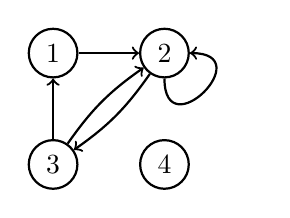
\begin{tikzpicture}
    \node [circle, thick, draw] at ( 45 : 1) (B) {2} ;
    \node [circle, thick, draw] at (135 : 1) (A) {1} ;
    \node [circle, thick, draw] at (225 : 1) (C) {3} ;
    \node [circle, thick, draw] at (315 : 1) (D) {4} ;
    \draw[thick,->] (A) -- (B) ;
    \draw[thick,->] (B) edge [in=0, out=270, looseness=5] (B) ;
    \draw[thick,->] (B) edge [bend left=10] (C) ;
    \draw[thick,->] (C) -- (A) ;
    \draw[thick,->] (C) edge [bend left=10] (B) ;
  \end{tikzpicture}
\end{center}
%
A common representation of graphs uses a pair of lists $(\ell_V, \ell_A)$, where $\ell_V$ is the list of vertex labels and $\ell_A$ the \emph{adjacency list} representing the edges as pairs of labels. For the above graph these would be $\ell_V = [1, 2, 3, 4]$ and $\ell_A = [(1,2), (2,2), (2,3), (3,2), (3,1)]$.
%
Thus we define the datatype of graphs as\sidenote{We use Haskell notation in which $[t]$ is the type of lists of
  elements of type~$t$, and $(t_1, t_2)$ is the cartesian product of types~$t_1$ and~$t_2$.}
%
\begin{lstlisting}[language=Haskell]
type Graph = ([Int], [(Int, Int)])
\end{lstlisting}
%
This is not yet a complete description of the intended representation, as there are representation invariants and conditions not expressed by the type:
%
\begin{itemize}
\item the order in which the vertices and edges are listed is not
  important,
\item every vertex and edge must be listed exactly once, and
\item the source and target of each edge must appear in the list of vertices.
\end{itemize}
%
Such conditions can be expressed in terms of a \defemph{realizability relation}
\begin{equation*}
  r \rz x
\end{equation*}
%
which tells which values~$r$ of the datatype correspond to which elements~$x$ of the set.
%
We read $r \rz x$ as ``$r$ realizes (implements, represents, witnesses) $x$''. In the above example we would write
%
\begin{equation*}
([1, 2, 3, 4], [(1,2), (2,2), (2,3), (3,2), (3,1)]) \rz G,
\end{equation*}
%
and also
%
\begin{equation*}
([3, 2, 1, 4], [(2,2), (1,2), (2,3), (3,2), (3,1)]) \rz G.
\end{equation*}
%
We also want to compute with the elements of $\mathsf{Graphs}$.
%
Programmers intuitively know what this mean, namely to implement, or realize, a map $f : \mathsf{Graphs} \to \mathsf{Graphs}$, is to give a program $p : \mathtt{graph} \to \mathtt{graph}$ which does to realizers what~$f$ does to elements: if $r \rz G$ then $p \, r \rz f(G)$. We say that~$f$ is \defemph{realized} or \defemph{tracked} by~$p$.

\section{Assemblies}
\label{sec:assemblies}

We now give a precise definition of the ideas presented in the previous section.

\begin{definition}
  An \defemph{assembly} over~$(\AA, \subAA)$ a tpca with a sub-tpca is a triple
  $\asm{S} = \xasm{S}$ where $S$ is a set, $|S|$ is a type in~$\AA$, and $\rz[S]$ is a relation between $\xAtyp{S}$ and~$S$
  satisfying: for every $x \in S$ there is $\R{x} \in \xAtyp{S}$ such that $\R{x} \rz[S] x$.

  An \defemph{assembly map} $f : \asm{S} \to \asm{T}$ between assemblies $\asm{S}$ and $\asm{T}$ is a map $f : S \to T$
  between the underlying sets for which there exists $\R{f} \in \subAtyp{|S| \to |T|}$, called a \defemph{realizer}
  of~$f$, satisfying: if $\R{x} \rz[S] x$ then $\defined{\R{f} \, \R{x}}$ and $\R{f} \, \R{x} \rz[T] f(x)$.
\end{definition}

We often use the same letter for an element and its realizer, but differentiate between them by using different fonts, for instance the elements $x$, $y$, $f$, $g$ would have realizers $\R{x}$, $\R{y}$, $\R{f}$, $\R{g}$, respectively.

There are many versions of realizability. Ours is known as \defemph{typed relative realizability}. It is \emph{typed}
because we used typed pcas. It is \emph{relative} because maps are realized relative to a choice of a sub-pca. In
typical cases, such as type~2 machines and the graph model from \cref{sec:type-2,sec:graph-model}, $\subAA$ is the
computable part of a topological pca~$\AA$, in accordance with the slogan
%
\begin{center}
  \emph{``Continuous data -- computable functions!''}
\end{center}

When $\subAA = \AA$ we write $\Asm{\AA}$ instead of $\Asm{\AA,\AA}$.

When $\AA$ is untyped the definition of an assembly simplifies a bit because we need mention the (trivial) types.

\begin{definition}
  An \defemph{assembly} over an untyped pca~$\AA$ is a pair $\asm{S} = (S, {\rz[S]})$ where $S$ is a set and $\rz[S]$ is a relation between~$\AA$ and~$S$, such that for every $x \in S$ there is $r \in A$ and $r \rz[S] x$.
\end{definition}

Assemblies and maps over $(\AA, \subAA)$ form a \defemph{category $\AsmA$}.
%
Indeed, if $f : \asm{S} \to \asm{T}$ and $g : \asm{T} \to \asm{U}$ are realized by $\R{f} \in \subAtyp{|S| \to |T|}$
and $\R{g} \in \subAtyp{|T| \to |U|}$, respectively, then their composition $g \circ f$ is realized by
$\tpcalam{x}{|S|}{r\,(q\,x)} = \combS\,(\combK\,r)\,(\combS\,(\combK\,q)\,(\combS\,\combK\,\combK))$.
%
The identity map $\id[S] : \asm{S} \to \asm{S}$ is realized by $\tpcalam{x}{|S|}{x} = \combS\,\combK\,\combK$. 
%
Composition is associative because it is just composition of maps.

\subsection{Modest sets}
\label{sec:modest-sets}

In the definition of assemblies, nothing prevents several elements from sharing a common realizer. We sometimes want
to prohibit such anomalies.

\begin{definition}
  An \defemph{modest} assembly $\asm{S}$, also called a \defemph{modest set},\sidenote{The terminology was suggested by Dana Scott. It refers to the fact that the cardinality of a modest set~$\asm{S}$ does not exceed the cardinality of $\xAtyp{S}$.} is an assembly in which elements do not share realizers:
  %
  \begin{equation*}
    \all{r}{\xAtyp{S}}{
      \all{x,y \in S}
      (r \rz[S] x \land r \rz[S] y \implies x = y)
    }.
  \end{equation*}
  %
  We let $\ModA$ be the full subcategory of $\AsmA$ on the modest sets.
\end{definition}

Most structures in computable mathematics turn out to be modest, but assemblies are needed also, and they form a richer category than the modest sets.

\subsection{First examples of assemblies}
\label{sec:examples-assemblies}

To gain a bit of intuition about assemblies, we look at several concrete examples. Unless stated otherise, we assume that all assemblies are constructed over a chosen pca with sub-pca $(\AA, \subAA)$.

\subsubsection{The unit assembly}
\label{sec:asm-unit}

Let $\unit$ be a type such that $\subAtyp{\unit}$ is inhabited.
It always exists, because there is at least one type $s$, and then
$\Atyp{s \to s \to s}$ contains $\combK_{s,s}$.
%
The \defemph{terminal assembly} $\one = (\set{\star}, \unit, {\rz[\one]})$ has the trivial realizability relation, $r \rz[\one] \star$ for all $r \in \subAtyp{t}$.

\begin{exercise}
  Show that $\one$ is the terminal object\sidenote{An object $T$ in a category is \defemph{terminal} when there is precisely one morphism to $T$ from every object.}
  in $\AsmA$. Conclude from this that a different choice of $\unit$ results in an isomorphic copy of~$\one$.
\end{exercise}

The morphisms $\one \to \asm{S}$ corresponds to those elements of~$S$ that are realized by elements of $\subAtyp{|S|}$. Indeed, if $f : \star \to S$ is realized by $\R{f} \in \subAtyp{\unit \to |S|}$ then $f \, \star$ is realized by $\R{f} \, t \in \subAtyp{|S|}$, for any $t \in \subAtyp{\unit}$. Conversely, if $a \in S$ is realized by $\R{a} \in \subAtyp{|S|}$ then $\star \mapsto a$ is $\tpcalam{x}{\unit}{\R{a}}$.

This may be a good moment to point out the difference between the \defemph{global points} of~$\asm{S}$, which is the set of morphisms $\one \to \asm{S}$, and the \defemph{underlying set~$S$} of~$\asm{S}$. Both induce functors $\AsmA \to \Set$, which need not be equivalent, unless $\AA = \subAA$.


\subsubsection{Natural numbers}
\label{sec:asm-natural-numbers}

Suppose $(\AA, \subAA)$ is an n-tpca. Let $\asm{N} = (\NN, \ttnat, {\rz[N]})$ be the set of natural numbers~$\NN$ realized by the numerals, for all $r \in \Atyp{\ttnat}$ and $n \in \NN$,
%
\begin{equation*}
  r \rz[N] n \iff
  r = \overline{n}.
\end{equation*}
%
The successor $n \mapsto n + 1$ is realized by~$\combSucc$, and $0 \in \mathbb{N}$ is a global point because $\numeral{0} \in \subAtyp{\ttnat}$.

The assembly $\mathbb{N}$ is the natural numbers object. Indeed, given an assembly $\asm{S}$ with $z \in \asm{S}$ realized by $\mathtt{z} \in \subAtyp{|S|}$, and $f : \asm{S} \to \asm{S}$, the unique map $\overline{f} : \asm{N} \to \asm{S}$ satisfying, for all $n \in \NN$,
%
\begin{equation*}
  \overline{f} \, 0 = 0
  \qquad\text{and}\qquad
  \overline{f} \, (n + 1) = f (\overline{f} n)
\end{equation*}
%
is realized by $\combRec \, \mathtt{z} \, \mathtt{f}$.


\subsubsection{Boolean, semidecidable, and classical truth values}
\label{sec:asm-two-element}

Let us work in the category $\Asm{\klone}$ over Kleene's first algebra and look at assembly structures on the set $2 = \set{0, 1}$.

First, we have the trivial structure, namely the assembly of \defemph{classical truth values} $\nabla 2 = (2, {\rz[\nabla 2]})$ -- the notation will become clear in \cref{sec:nabla}, and the nomenclature a bit later -- with the trivial realizability relation $n \rz[\nabla \two] b$ for all $k \in \NN$ and $b \in 2$.

Second, we have the assembly of \defemph{Boolean values} $\two = (2, {\rz[2]})$ where $n \rz[2] b$ if, and only if $n = b$.

The assemblies $\nabla 2$ and $\two$ are \emph{not} isomorphic because every assembly map $\nabla 2 \to \two$ is constant, although the identity map is an assembly map $\two \to \nabla 2$.

There are still more two-element assemblies, for instance the assembly of \defemph{semidecidable values} $\asm{S} = (2, {\rz[S]})$ given by
%
\begin{equation*}
  n \rz b \iff
  (\divergent{\pr{n}{n}} \land b = 0) \lor (\defined{\pr{n}{n}} \land b = 1).
\end{equation*}
%
Again, the identity map is realized as an assembly map $\two \to \asm{S}$, but not the other way around.

\begin{exercise}
  Why is identity not realized as a map $\asm{S} \to \two$?
\end{exercise}


\subsubsection{Real numbers}
\label{sec:asm-real-numbers}

As our third example we ask how to equip the real numbers with a realizability structure. Here we give the correct answer, but leave it unexplained for the time being.

We work with an nr-tpca $\AA$ with a sub-n-tpca $\subAA$. Intuitively speaking, a realizer for $x \in \RR$ should allow us to compute arbitrarily good approximations of~$x$, so we define the relation $\rz[R]$ between $\Atyp{\ttnat \to \ttnat \times \ttnat \times \ttnat}$ by stipulating that $\R{x} \rz[R] x$ holds if, and only if,
%
\begin{equation*}
  \all{k \in \NN} \some{a, b, c \in \NN}
  \R{x} \, \overline{k} = (\overline{a}, \overline{b}, \overline{c})
  \land |x - \frac{a - b}{1 + b}| < 2^{-k}.
\end{equation*}
%
The triple of numbers $(a, b, c)$ is just a clumsy way of encoding the rational $\frac{a - b}{c}$, so in essence $\R{x}$ computes a sequence of rationals such that the $k$-th term is within~$2^{-k}$ of~$x$.

The assembly of real numbers $\asm{R} = (R, \ttnat \to \ttnat \times \ttnat \times \ttnat, {\rz[R]})$ has as its underlying set the realized reals
%
\begin{equation*}
  R = \set{x \in \RR \such \some{\R{x} \in \Atyp{\ttnat \to \ttnat \times \ttnat \times \ttnat}} \R{x} \rz[R] x}.
\end{equation*}
%
Which reals are so realized depends on the choice of~$\AA$. For example, first Kleene algebra realizes the \defemph{Turing computable reals}, whereas the second Kleene algebra realizes all reals.

\subsection{The constant assemblies}
\label{sec:nabla}

The extreme case of elements sharing the same realizer happens when
all elements of a set share all realizers. Assemblies with this
property are called the \defemph{constant assemblies}.

Let $t$ be a type such that $\subAtyp{t}$ is inhabited. Such a type
always exists, because there is at least one type $s$, and then
$\Atyp{s \to s \to s}$ contains $\combK_{s,s}$. Given any set $X$, let
%
\begin{equation*}
  \nabla X = (X, t, {\rz[\nabla X]})
\end{equation*}
%
be the assembly whose underlying set is~$X$ and the realizability relation is trivial, i.e., $r \rz[\nabla X] x$ for all $x \in X$ and $r \in A_t$.

If $f : X \to Y$ is any map between sets~$X$ and~$Y$ then~$f$ is a morphism $\nabla f : \nabla X \to \nabla Y$ because it is tracked by $\tpcalam{x}{t}{x}$. Thus~$\nabla$ is a functor
%
\begin{equation*}
  \nabla : \Set \to \AsmA.
\end{equation*}
%
Up to natural isomorphism, $\nabla$ is independent of the choice of
type~$t$. We will study the properties of $\nabla$ later on. For now
we notice that $\nabla$ is full and faithful, which means that
$\AsmA$ contains the category of sets as a full
subcategory.

The functor $\nabla$ is devoid of any computational content because it
represents a set~$X$ by a trivial realizability relation which conveys
no information at all about the elements of~$X$. Consequently, from
the realizers we cannot compute anything interesting regarding~$X$.

\begin{exercise}
  Let $\Gamma : \AsmA \to \Set$ be the forgetful functor which assigns to an assembly its underlying set, and to an
  aseembly map the underlying set-theoretic function. Show that~$\Gamma$ is left adjoint to~$\Delta$.
\end{exercise}

\section{Equivalent formulations}
\label{sec:equivalent-formulations}

Assemblies and modest sets have several equivalent formulations, which were formulated by different communities for particular choices of $(\AA, \subAA)$, each using their own notation and terminology. In this section we review the equivalent formulations, and in \cref{sec:schools} show how various ``schools of computable mathematics'' arise as special instances.

\subsection{Existence predicates}
\label{sec:existence-predicates}

A realizability relation $\rz[S]$ is a subset of $\xAtyp{S} \times S$. By transposition it may be equivalently expressed
as a map $\Ex_S : S \to \pow{\xAtyp{S}}$. The correspondence is
%
\begin{equation*}
  \R{x} \rz[S] x \iff \R{x} \in \Ex_S(x).
\end{equation*}
%
Because every $x$ is realized by something, $\Ex_S(x)$ always contains at least one element. Thus an assembly $\xasm{S}$ may be equivalently presented as a triple $(S, |S|, \Ex_S)$ where $\Ex_S : S \to \pow{\xAtyp{S}}$ is a map, called the \defemph{existence predicate}, such that $\Ex_S(x)$ contains at least one element for every $x \in S$. The name suggests that the elements of $\Ex_S(x)$ are computational witnesses for ``existence of~$x$''.

An assembly $S$ is modest if, and only if, $\Ex_S(x) \cap \Ex_S(y) \neq \emptyset$ implies $x = y$.

Under this formulation a map $f : \asm{S} \to \asm{T}$ is realized if there exists $\R{f} \in \subAtyp{|S| \to |T|}$ such that, for all $x \in S$ and $\R{x} \in \Ex_S(x)$, $\defined{\R{f}\,\R{x}}$ and $\R{f}\,\R{x} \in \Ex_T(f(x))$.

\subsection{Representations}
\label{sec:representations}

By transposing $\rz[S]$ the other way around we obtain \defemph{representations}. Suppose first that $S$ is a modest set. Since every realizer $r \in \xAtyp{S}$ realizes at most one $x \in S$, we may define a partial map $\delta_S : \xAtyp{S} \parto S$ by
%
\begin{equation*}
  \delta_S(r) = x \iff r \rz[S] x.
\end{equation*}
%
The map $\delta_S$ is surjective because every $x \in S$ is realized, but it need not be defined everywhere. The triple $(S, |S|, \delta_S)$ uniquely describes the modest set~$S$. The map $\delta_S$ is called a \defemph{representation} of~$S$.

A map $f : S \to T$ is realized or tracked by $\R{f} \in \subAtyp{|S| \to |T|}$ when, for all $\R{x} \in \dom{\delta_S}$, $\defined{\R{f}\,\R{x}}$ and $\delta_T(\R{f}\,\R{x}) = f(\delta_S(x))$.

Representations and realized maps form a category~$\Rep{\AA,\subAA}$, which is equivalent to $\Mod{\AA, \subAA}$.

When we transpose $\rz[S]$ for a a general assembly $\asm{S}$ the result is a \defemph{multi-valued representation}, which is a map $\delta_S : \xAtyp{S} \multito \pow{S}$ that takes each $r \in \xAtyp{S}$ to the (possibly empty) set of elements it realizes,
%
\begin{equation*}
  \delta_S(r) = \set{ x \in S \such r \rz[S] x}.
\end{equation*}
%
The map is surjective in the sense that for every $x \in S$ there is $r \in \xAtyp{S}$ such that $x \in \delta_S(r)$.

To summarize, there are three ways of specifying the realizability structure of an assembly: with a realizability relation $\rz[S]$, an existence predicate~$\Ex_s$, and a multi-valued representation $\delta_S$. Each determines the other two by
%
\begin{equation*}
  r \rz[S] x \iff
  r \in \Ex_S(x) \iff
  x \in \delta_S(r).
\end{equation*}


\subsection{Partial equivalence relations}
\label{sec:pers}

This formulation only works for modest sets. With each modest set~$S$ we may associate a partial equivalence relation\sidenote{A \defemph{partial equivalence relation} is a transitive symmetric relation.} (per) $\per_S$ on $\xAtyp{S}$ which relates~$q$ and~$r$ when they realize the same element:
%
\begin{equation*}
  q \per_S r \iff
  \some{x \in S} q \rz[S] x \land r \rz[S] x.
\end{equation*}
%
The pair $(|S|, {\per_S})$ suffices for the reconstruction of the
original modest set, up to isomorphism, which we show next.

Let $(\AA, \subAA)$ be a tpca with a sub-tpca. A \defemph{partial
  equivalence relation} on~$\AA$ is a pair $S = (|S|, {\per_S})$ where
$|S|$ is a type and $\per_S$ is a transitive and symmetric
relation on $\xAtyp{S}$. A realizer $r \in \xAtyp{S}$ is \defemph{total} if
$r \per_S r$. The set of total realizers is denoted by $\|S\| = \set{r
  \in \xAtyp{S} \such r \per_S r}$. Each $r \in \|S\|$ determines
the equivalence class $[r]_S = \set{q \in \xAtyp{S} \such r \per_S q}$.

An \defemph{extensional realizer} between pers $S$ and $T$ is $p \in
\subAtyp{|S| \to |T|}$ such that, for all $q, r \in \xAtyp{S}$, if $q
\per_S r$ then $\defined{p\,q}$, $\defined{p\,r}$, and $p\,q \per_T
p\,r$. Extensional realizers $p$ and $p'$ are \defemph{equivalent} when
$q \per_S r$ implies $p\,q \per_T p'\,r$.

Pers and equivalence classes of extensional realizers form a category
$\Per{\AA, \subAA}$ whose objects are pers on~$\AA$ and morphisms are
equivalence classes of extensional realizers. The composition of $[p]
: S \to T$ and $[q] : T \to U$ is $[q \circ p] : S \to U$ where $q
\circ p = \tpcalam{x}{|S|}{q\,(p\,x)}$. The identity morphism
$\id[S] : S \to S$ is represented by $\tpcalam{x}{|S|} x$. It
is easy to check that this forms a category.

Let $S$ and $T$ be pers over $(\AA, \subAA)$. A morphism between them
may be alternatively described as a function $f : \|S\|/{\per_S} \to
\|T\|/{\per_T}$ between the equivalence classes for which there exists
a realizer $p \in \subAtyp{|S| \to |T|}$ that tracks it: for every
equivalence class $[r]_S$, $\defined{p\,r}$ and $[p\,r]_T = f([r]_S)$.

\begin{lemma}
  \label{lemma:iso-assembly}
  %
  Suppose $\asm{S}$ is an assembly, $T$ is a set, and $f : T \to S$ is
  a bijection. Then $\asm{S}$ is isomorphic to $\asm{T} = (T, |S|,
  {\rz[T]})$ where $r \rz[T] x$ is defined as $r \rz[S] f(x)$.
\end{lemma}


\begin{proof}
  The map $f$ is a morphism from $\asm{S}$ to $\asm{T}$ because it is
  tracked by~$\tpcalam{x}{|S|}{x}$. Similarly, $\inv{f}$ is a
  morphism because it is also tracked by the same realizer. Obviously,
  $f$ and $\inv{f}$ are inverses of each other.
\end{proof}


\begin{proposition}
  The categories $\Mod{\AA, \subAA}$ and $\Per{\AA, \subAA}$ are
  equivalent.
\end{proposition}

\begin{proof}
  A modest set $\xasm{S}$ determines a per $(S, {\per_S})$,
  as described above. A morphism $f : S \to T$ which is tracked by $p
  \in \subAtyp{|S| \to |T|}$ determines a morphism of pers $[p] : (S,
  {\per_S}) \to (T, {\per_T})$. This defines a functor $F : \Mod{\AA,
    \subAA} \to \Per{\AA, \subAA}$.

  In the other direction the functor $G : \Per{\AA, \subAA} \to
  \Mod{\AA, \subAA}$ sends a per $(|T|, {\per_T})$ to the modest set
  $(\|T\|/{\per_T}, |T|, {\rz[T]})$ whose realizability relation is
  %
  \begin{equation*}
    r \rz[T] [q] \iff r \per_T q.
  \end{equation*}
  %
  A morphism $[p] : (S, {\per_S}) \to (T, {\per_T})$ is mapped to the
  map $G [p] : \|S\|/{\per_S} \to \|T\|/{\per_T}$, defined by $G [p]
  [r]_S = [p\,r]_T$, which is obviously tracked by~$p$.

  The functors $F$ and $G$ form an equivalence of categories. The
  composition $F \circ G$ is actually equal to identity, as is easily
  verified. A modest set~$\xasm{S}$ is isomorphic to
  $G(F(S))$ by \cref{lemma:iso-assembly} applied to the bijection
  which takes an $x \in S$ to $[r]_{G(F(S))}$, where $r \in \xAtyp{S}$
  is any realizer such that $r \rz[S] x$. We leave the verification
  that the isomorphisms are natural as exercise.
\end{proof}


\subsection{Equivalence relations}
\label{sec:ers}

A per $(|S|, {\per_S})$ may be viewed as an equivalence relation on
$\|S\| = \set{r \in \xAtyp{S} \such r \per_S r}$. This gives us yet
another equivalent formulation of modest sets, this time in terms of
equivalence relations.

The category $\Er{\AA, \subAA}$ of equivalence relations has as objects triples $(S, |S|, {\equiv_S})$ where $|S|$ is a
type, $S \subseteq \xAtyp{S}$, and $\equiv_S$ is an equivalence relation on~$S$. As in the case of pers, a morphism
$(S, |S|, {\equiv_S}) \to (T, |T|, {\equiv_T})$ is represented by an extensional realizer
$p \in \subAtyp{|S| \to |T|}$.

The difference between pers and equivalence relations is mostly a
bureaucratic one. Nevertheless, it is useful to know about $\Er{\AA,
  \subAA}$ because sometimes we can describe it in enlightening
alternative ways, e.g., in \cref{sec:equilogical-spaces} we
describe pers on the graph model as equivalence relations on
topological spaces.

\section{Applicative functors}
\label{sec:applicative-functors}


\index{functor!induced by applicative morphism}%
\index{applicative!morphism!functor induced by}%

Categories of assemblies themselves form a category whose morphisms are functors induced by simulations, known as \emph{applicative functors}. These were defined and studied by John Longley~\cite{Longley:94}, and are the appropriate notion of morphisms of assemblies, as well as realizability toposes. We review their definition and several basic results about them, which we cannot do without assuming some knowledge of basic category theory.

A simulation $\rho: (\EE, \subEE) \pcato (\FF, \subFF)$ induces an \defemph{applicative functor}
%
\begin{equation*}
  \ff{\rho}: \Asm{\EE, \subEE} \longrightarrow \Asm{\FF, \subFF}
\end{equation*}
%
which maps an assembly $\asm{S} = (S, {\rz[S]})$ over $(\EE, \subEE)$ to the assembly
$\ff{\rho} \, \asm{S}$ over $(\FF, \subFF)$, whose underlying set is $S$ and
%
\begin{align*}
  q \rz[\ff{\rho \asm{S}}] x
  \iff \some{r \in \EE} q \in \rho[r] \land r \rz[S] x.
\end{align*}
%
That is, $\ff{\rho}$ replaces realizers in~$\EE$ with their simulations in~$\FF$.

Suppose $r \in \subFF$ is a realizer for~$\rho$. An assembly map $f: \asm{S} \to \asm{T}$, realized by $\mathtt{f} \in \subEE$, is mapped by $\ff{\rho}$ to the same underlying map $\ff{\rho}\,f = f$, which is realized by $r \, \mathtt{g}$ for any $\mathtt{g} \in \rho[\mathtt{f}]$.

\begin{exercise}
  Prove that and applicative functor induced by a \emph{discrete} simulation restricts to modest sets.
\end{exercise}

The properties of the induced applicative functor depend on the properties of the simulation, as follows. (We presume existence of categorical structure on assemblies which will only be established in \cref{cha:categ-structure}.)

\begin{proposition}
  \label{th:applicative_functor_properties}%
  %
  Let $\rho: (\EE, \subEE) \pcato (\FF, \subFF)$ be a simulation.
  % 
  \begin{enumerate}
  \item
    %
    The functor $\ff{\rho}$ is faithful  and it preserves finite limits.
  \item
    %
    If $\rho$ is projective then $\ff{\rho}$ preserves projective objects.
  \item
    %
    If $\rho$ is decidable then $\ff{\rho}$ preserves finite colimits and the natural numbers object.
  \end{enumerate}
\end{proposition}

\begin{proof}
  The functor $\ff{\gamma}$ preserves finite limits
  by~\cite[Proposition~2.2.2]{Longley:94}. It is faithful
  because it acts trivially on morphisms.
  %
  For the second claim see~\cite[Theorem~2.4.12]{Longley:94}, and for the third one~\cite[Theorem~2.4.19]{Longley:94}.
\end{proof}

Adjunctions and equivalences between simulations carry over to the induced morphisms.

\begin{theorem}
  \label{th:applicative_adjunction_functor_adjunction}%
  Consider simulations
                                %
  \begin{align*}
    \delta &: (\EE, \subEE) \pcato (\FF, \subFF),
    &
    \gamma &: (\FF, \subFF) \pcato (\EE, \subEE).
  \end{align*}
                                %
  \begin{enumerate}
  \item If $\gamma \dashv \delta$ is an adjoint pair, then
    $\ff{\gamma} \dashv \ff{\delta}$ is an adjunction of functors.
    %
    \index{adjunction!induced by simulation adjunction}%
    %
  \item If $\gamma \dashv \delta$ is an adjoint inclusion then the counit of the adjunction $\ff{\gamma} \dashv \ff{\delta}$ is a natural isomorphism.
    %
  \item If $\gamma \dashv \delta$ is an adjoint retraction then the unit of the adjunction $\ff{\gamma} \dashv \ff{\delta}$ is a natural isomorphism.
  \item If $\gamma$ and $\delta$ form an equivalence, then so do $\ff{\gamma}$ and
    $\ff{\delta}$.
  \end{enumerate}
\end{theorem}

\begin{proof}
  The first three claims are subsumed by the easy part of~\cite[Proposition 2.5.9]{Longley:94}, except that we are using simulations on pcas with sub-pcas. Also, we are restricting attention to categories of assemblies rather than realizability toposes, but this is not a problem because by applicative functors on realizability toposes restrict to assemblies.

  That equivalences of simulations induce equivalences of categories is shown in~\cite[Theorem 2.5.6]{Longley:94}.
\end{proof}

The construction of assemblies and induced applicative functors extends to a 2-functor between 2-categories. Indeed, given $\gamma, \delta : (\EE, \subEE) \pcato (\FF, \subFF)$ such that $\gamma \preceq \delta$, there is an induced natural transformation $\zeta : \ff{\gamma} \natto \ff{\delta}$ defined by
%
\begin{equation*}
  \zeta_{\asm{S}} = \id[S] : \ff{\gamma}\,\asm{S} \to \ff{\delta}\,\asm{S}.
\end{equation*}
%
This is a valid definition, for if $t \in \subFF$ is a translation witnessing $\gamma \preceq \delta$, then $t$ tracks every $\zeta_{\asm{S}}$, and the naturality condition is trivial.

An applicative functor induced by $\rho : (\EE, \subEE) \pcato (\FF, \subFF)$ commutes up to natural isomorphism with the constant assembly functor~$\nabla$ from \cref{sec:nabla},
%
\begin{equation*}
  \xymatrix{
    {\Asm{\EE, \subEE}}
    \ar[rr]^{\ff{\rho}}
    & &
    {\Asm{\FF, \subFF}}
    \\
    & {\Set}
    \ar[ur]_{\nabla}
    \ar[ul]^{\nabla}
  }
\end{equation*}
%
as well as with the underlying set functor~$\Gamma$,
%
\begin{equation*}
  \xymatrix{
    {\Asm{\EE, \subEE}}
    \ar[rr]^{\ff{\rho}}
    \ar[dr]_{\Gamma}
    & &
    {\Asm{\FF, \subFF}}
    \ar[dl]^{\Gamma}
    \\
    & {\Set}
  }
\end{equation*}
%
See \cite[Proposition 2.2.4]{Longley:94} for the proof.

%%% Local Variables: 
%%% mode: latex
%%% TeX-master: "notes-on-realizability"
%%% End: 

\chapter{The category-theoretic structure}
\label{cha:categ-structure}


In Chapter~\ref{chap:realizability} we defined assemblies as our basic
structures of interest. To learn more about them we study which
operations on assemblies are supported by the category $\AsmA$. It
turns out that there is not only a rich collection of constructions
available, but also an interpretation of first-order logic that
assigns to a logical formula its computational meaning.


In their everyday lives mathematicians use a limited set of
constructions on sets: products, disjoint sums, subsets, quotient
sets, images, function spaces, inductive and coinductive definitions,
powersets, unions, intersections, and complements. For all of these,
except powersets, there are analogous constructions of assemblies.
Therefore, if we need a computable version of a given mathematical
structure, may just mimic its set-theoretic definition in the
category of assemblies.

\section{The cartesian structure}
\label{sec:cartesian-structure}

A construction which makes a new set, space, or an algebraic structure
from old ones is usually characterized by a \emph{universal property}
which determines it up to isomorphism. The universal property is
shared among versions of the same construction in different
categories. We start slowly with an easy one, the binary product.

Recall the definition of a \defemph{(binary) product} in a category: the
product of objects $S$ and $T$ is an object $P$ with morphisms $p_1 :
P \to S$ and $p_2 : P \to T$, satisfying the following universal
property: for all morphisms $f : U \to S$ and $g : U \to T$ there is a
unique morphism $h : U \to P$ making the following diagram commute:
%
\begin{equation*}
  \xymatrix@+1em{
    &
    {U}
    \ar[ld]_{f}
    \ar[d]^h
    \ar[rd]^{g}
    &
    \\
    {S}
    &
    {P}
    \ar[l]^{p_1}
    \ar[r]_{p_2}
    &
    {T}
  }
\end{equation*}
%
The products $(P, p_1, p_2)$ is determined uniquely up to a unique
isomorphism. For suppose we had another product $(Q, q_1, q_2)$ of~$S$
and~$T$. By the universal property of $P$ there is a map $h : P \to Q$
such that $p_1 \circ h = q_1$ and $p_2 \circ h = q_2$. Similarly, by
the universal property of~$Q$ there is $k : Q \to P$ such that $q_1
\circ k = p_1$ and $q_2 \circ k = p_2$. Now $h \circ k$ satisfies
%
\begin{equation*}
  p_1 \circ h \circ k = q_1 \circ k = p_1
  \qquad\text{and}\qquad
  p_2 \circ h \circ k = q_2 \circ k = p_2.
\end{equation*}
%
Since $\id_P$ also satisfies $p_1 \circ \id_P = p_1$ and $p_2 \circ
\id_P = p_2$, it follows by the uniqueness condition of the universal
property that $h \circ k = \id_P$. A similar argument shows that $k
\circ h = \id_Q$, hence $P$ and $Q$ are isomorphic.

A category \defemph{has binary products} if every pair of objects has a
binary product. In most cases we can actually provide an operation
$\times$ which maps a pair of objects $S$, $T$ to a specifically given
product $S \times T$ with corresponding projections. The unique map
$h$ determined by $f$ and $g$ is denoted by $\pair{f,g}$.

In the category~$\Set$ the product is just the usual cartesian product
of sets. In assemblies we need to worry about the underlying types and
realizability relations. Let us verify that the product of assemblies
$\asm{S}$ and $\asm{T}$ is the assembly
%
\begin{equation*}
  \asm{S} \times \asm{T} =
  (S \times T, |S| \times |T|, {\rz_{S \times T}})
\end{equation*}
%
with the realizability relation
%
\begin{equation*}
  \combPair\;q\;r \rz_{S \times T} (x,y)
  \iff
  q \rz_S x
  \land
  r \rz_T y.
\end{equation*}
%
and the projection maps $\pi_1 : S \times T \to S$, $\pi_1 : (x,y)
\mapsto x$, and $\pi_2 : S \times T \to T$, $\pi_2 : (x,y) \mapsto y$,
which are realized by $\combFst$ and $\combSnd$, respectively.
%
To see that $(\asm{S} \times \asm{T}, \pi_1, \pi_2)$ has the universal
property, suppose $f : \asm{U} \to \asm{S}$ and $g : \asm{U} \to
\asm{T}$ are realized by $\R{f} \in \comp{A}_{|U| \to |S|}$ and $\R{g}
\in \comp{A}_{|U| \to |T|}$, respectively. There is a unique map $h :
U \to S \times T$ for which $f = \pi_1 \circ h$ and $g = \pi_2 \circ g$,
namely $h(u) = \pair{f,g}(u) = (f(u), g(u))$. We only need a realizer
for~$h$, and $\R{h} =
\pcalam{\annot{u}{|U|}}{\combPair\;(\R{f}\;u)\;(\R{g}\;u)}$ does the
job:
%
\begin{multline*}
  \R{u} \rz_U u
  \implies
  \R{f}\;\R{u} \rz_S f(u)
  \land
  \R{g}\;\R{u} \rz_T g(u)
  \implies {} \\
  \combPair\; (\R{f}\;\R{u})\; (\R{g}\;\R{u}) \rz_{S \times T} (f(u), g(u))
  \iff
  \R{h}\;\R{u} \rz_{S \times T} h(u).
\end{multline*}

Once we have binary products we may form $n$-ary products $S_1 \times
\cdots \times S_n$ for $n \geq 1$ by repeatedly forming binary
products. The case $n = 0$ corresponds to the \defemph{terminal object},
which is an object $\one$ such that for every object~$S$ there is
exactly one morphism $S \to \one$. In the category of sets the
terminal object is (any) singleton set, say $\one = \set{\star}$. Then
$\nabla \one$ is the terminal assembly, since for any assembly
$\asm{S}$ the only map $S \to \one$ is realized. We denote the
terminal assembly as $\one$.

We may also ask whether $\AsmA$ has infinite products. The answer
depends on the underlying TPCAs $(\AA, \compAA)$. We state without
proof that $\Asm{\Scott, \comp{\Scott}}$ and $\Asm{\Baire,
  \comp{\Baire}}$ have countable products, whereas $\Asm{\NN}$ does
not.

Products are a special case of categorical limits. Two other common
kinds of limits are equalizers and pullbacks. An \defemph{equalizer} of a
pair of morphisms $f, g : S \to T$ is an object $E$ with a morphism $e
: E \to S$ such that $e$ equalizes $f$ and $g$, which means that $f
\circ e = g \circ e$, and the following universal property is
satisfied: if $k : K \to S$ also equalizes $f$ and $g$ then there
exists a unique morphism $i : K \to E$ such that $k = e \circ i$:
%
\begin{equation*}
  \xymatrix@+1em{
    {E}
    \ar[r]^{e}
    &
    {S}
    \ar@<+0.25em>[r]^{f}
    \ar@<-0.25em>[r]_{g}
    &
    {T}
    \\
    {K}
    \ar[u]^{i}
    \ar[ru]_{k}
    & & 
  }
\end{equation*}
%
Think of $E$ as the solution-set of equation $f(x) =
g(x)$.\sidenote{If we have a system of equations $f_i(x) = g_i(x)$, $i
  = 1, \ldots, n$, then we may express them as a single vector
  equation $f(x) = g(x)$ where $f(x) = (f_1(x), \ldots, f_n(x))$ and
  $g(x) = (g_1(x), \ldots, g_n(x))$. Equalizers are thus an abstract
  formulation of the notion ``solution of a system of equations''.}
Indeed, in the category of sets the equalizer of functions $f, g : S
\to T$ is the subset $E = \set{x \in S \such f(x) = g(x)}$ and $e : E
\to S$ is the subset inclusion. In the category of assemblies we need
to augment this with realizers. The equalizer of $f, g : \asm{S} \to
\asm{T}$ is
%
\begin{equation}
  \label{eq:asm-equalizer}%
  \asm{E} =
  (\set{x \in S \such f(x) = g(x)},
   |S|,
   {\rz_E})
\end{equation}
%
where $\R{x} \rz_E x$ if, and only if, $\R{x} \rz_S x$. The map $e : E
\to S$ is the subset inclusion, $e(x) = x$. It is realized by
$\xpcalam{\annot{x}{|S|}}{x}$. Clearly, $e$ equalizes~$f$ and~$g$. We
leave the verification of the universal property as exercise.

A \defemph{pullback}, sometimes called \defemph{fibered product}, is a
combination of product and equalizer. Given morphisms $f : S \to U$
and $g : T \to U$, the pullback of $f$ and $g$ is an object $P$ with
morphisms $p_1 : P \to S$ and $p_2 : P \to T$ such that $f \circ p_1 =
g \circ p_2$. Furthermore, if $q_1 : Q \to S$ and $q_2 : Q \to T$ are
such that $f \circ q_1 = g \circ q_2$ then there is a unique $i : Q
\to P$ which makes the following diagram commute:
%
\begin{equation*}
  \xymatrix@+0.5em{
    {Q}
    \ar[dr]^{i}
    \ar@/_1em/[ddr]_{q_2}
    \ar@/^1em/[rrd]^{q_1}
    &
    &
    \\
    &
    {P} \pbcorner
    \ar[r]^{p_1}
    \ar[d]_{p_2}
    &
    {S}
    \ar[d]^{f}
    \\
    &
    {T}
    \ar[r]_{g}
    &
    {U}
  }
\end{equation*}
%
The fact that $P$ is a pullback is traditionally marked in a diagram
with the ``corner'' symbol. In the category of assemblies the pullback
of $f : \asm{S} \to \asm{U}$ and $g : \asm{T} \to \asm{U}$ is the
assembly
%
\begin{equation*}
  \asm{P} = (\set{(x,y) \in S \times T \such f(x) = g(y)}, |S| \times
  |T|, {\rz_P})
\end{equation*}
%
where $\combPair\;\R{x}\;\R{y} \rz_P (x,y)$ if, and only if, $\R{x}
\rz_S x$ and $\R{y} \rz_T y$.

Finite products, the terminal object, equalizers, and pullbacks are
special cases of \defemph{finite limits}. A category which has all finite
limits is called \defemph{cartesian} or \defemph{finitely
  complete}.\sidenote{We do not like much the still older terminology
  \emph{left exact} or just \emph{lex}.}

\begin{proposition}
  \label{prop:asm-cartesian}%
  The categories $\AsmA$ and $\Mod{\AA, \compAA}$ are cartesian.
\end{proposition}

\begin{proof}
  It is well known that every finite limit may be constructed as a
  combination of a finite product and an equalizer, hence $\AsmA$ is
  cartesian. It is easy to verify that finite products and equalizers
  of modest assemblies are again modest, therefore $\Mod{\AA,
    \compAA}$ is cartesian.
\end{proof}


%%%%%%%%%%%%%%%%%%%%%%%%%%%%%%%%%%%%%%%%%%%%%%%%%%
\section{Cocartesian structure}
\label{sec:cocartesian-structure}


Colimits are the dual of limits. In particular, the dual of products,
terminal object, equalizers, and pullbacks are respectively
coproducts, initial object, coequalizers, and pushouts. We study which
of these exist in~$\AsmA$.

First we discuss (binary) coproducts of sets, also known as disjoint
sums. For some reason there does not seem to be a well-established and
practical notation for these, possibly because the related union
operation is taken as primitive in set theory. The disjoint sum of
sets~$S$ and~$T$ is usually defined as
%
\begin{equation*}
  S + T = (\set{0} \times S) \cup (\set{1} \times T).
\end{equation*}
%
The canonical injections $\iota_1 : S \to S + T$ and $\iota_2 : T \to
S + T$ are the maps $x \mapsto (0,x)$ and $y \mapsto (1,x)$,
respectively. A slight notational inconvenience arises when want to
define a map $f : S + T \to U$ by cases $f_1 : S \to U$ and $f_2 : T
\to U$. One possibility is to write
%
\begin{equation*}
  f(u) =
  \begin{cases}
    f_1(x) & \text{if $u = (0,x)$,}\\
    f_2(y) & \text{if $u = (1,y)$,}
  \end{cases}
\end{equation*}
%
but this is seen rarely. In practice mathematicians prefer to assume,
or shall we say \emph{pretend}, that the sets~$S$ and~$T$ are disjoint
and just write $S + T = S \cup T$. This allows us to get rid of the
encoding by pairs,
%
\begin{equation*}
  f(u) =
  \begin{cases}
    f_1(u) & \text{if $u \in S$,}\\
   f_2(u) & \text{if $u \in T$.}
  \end{cases}
\end{equation*}
%
Unlike people, computers do not pretend, and so as computer scientists
we need notation that is actually correct. However, it is unnecessary
to write the elements of a disjoint sum as uninformative pairs $(0,x)$
and $(1,y)$. Instead, we simply take the injections $\iota_1$ and
$\iota_2$ as \emph{labels} that indicate which part of a disjoint sum
we are referring to. Thus, every element of $S + T$ is either of the
form $\iota_1(x)$ for a unique $x \in S$, or $\iota_2(y)$ for a unique
$y \in T$.\sidenote{If you feel the urge to really encode everything
  with sets, you can still define $\iota_1(x) = (0, x)$ and
  $\iota_2(y) = (1, y)$ but then forget the definition.} In a specific
case we may choose different, descriptive names for the injections.

Definition by cases is a primitive concept involving disjoint sums
which deserves its own notation, preferably one that fits on a single
line. We may mimic Haskell and write
%
\begin{equation*}
  \case{e}{\iota_1(x)}{e_1}{\iota_2(y)}{e_2}.
\end{equation*}
%
Read this as ``if $e$ is of the form $\iota_1(x)$ then $e_1$, else if
$e$ is of the form $\iota_2(y)$ then $e_2$''. The variables $x$ and
$y$ are bound in $e_1$ and $e_2$, respectively. The definition of $f$
above would be written as
%
\begin{equation*}
  f(u) = \case{u}{\iota_1(x)}{f_1(x)}{\iota_2(y)}{f_2(y)},
\end{equation*}
%
or spanning several lines
%
\begin{equation*}
  f(u) = \xcase{u}{\iota_1(x)}{f_1(x)}{\iota_2(y)}{f_2(y).}
\end{equation*}
%
We shall use this notation. Let us mention that in Haskell $\iota_1$
and $\iota_2$ are called $\mathtt{Left}$ and $\mathtt{Right}$,
respectively.

In a general category a \defemph{(binary) coproduct} of objects~$S$
and~$T$ is an object $C$ with morphisms $\iota_1 : S \to C$ and
$\iota_2 : T \to C$ such that, for all morphisms $f : S \to U$ and $g
: T \to U$ there exists a unique $h : C \to U$ such that the following
diagram commutes:
%
\begin{equation*}
  \xymatrix@+1em{
    &
    {U}
    &
    \\
    {S}
    \ar[r]_{\iota_1}
    \ar[ru]^{f}
    &
    {C}
    \ar[u]^{h}
    &
    {T}
    \ar[l]^{\iota_2}
    \ar[lu]_{g}
  }
\end{equation*}
%
Notice that we have exactly reversed all the morphisms with respect to
the definition of products. We write the coproduct of $S$ and $T$ as
$S + T$ when it is given as an operation, and the unique morphism~$h$
as~$[f,g]$.

Whether assemblies $\AsmA$ have binary coproducts is an interesting
question. The answer seems to depend on the structure of the
underlying TPCAs.

\begin{definition}
  A TPCA~$\AA$ with \defemph{sums} is a TPCA with a binary operation $+$
  on the types such that, for all types $s$, $t$, and $u$ there exist
  constants
  %
  \begin{align*}
    \combLeft_{s,t} &\in \Atyp{s \to (s + t)} \\
    \combRight_{s,t} &\in \Atyp{t \to (s + t)} \\
    \combCase_{s,t,u} &\in \Atyp{(s + t) \to (s \to u) \to (t \to u) \to u}
  \end{align*}
  %
  satisfying, for all $x$, $y$, $f$, $g$ of appropriate types,
  %
  \begin{align*}
    \defined{\combLeft_{s,t}\;x} &, \\
    \defined{\combRight_{s,t}\;y} &,\\
    \combCase_{s,t,u}\;(\combLeft_{s,t}\;x)\;f\;g &\klgeq f\;x, \\
    \combCase_{s,t,u}\;(\combRight_{s,t}\;y)\;f\;g &\klgeq g\;y.
  \end{align*}
  %
  We say that the elements $\combLeft$, $\combRight$, and $\combCase$
  are \emph{suitable} for sums when they satisfy these properties.

  A \defemph{sub-TPCA with sums} is a sub-TPCA $\compAA$ of~$\AA$ such
  that there exists $\combLeft$, $\combRight$, $\combCase$
  in~$\compAA$ suitable for sums in $\AA$.
\end{definition}

\begin{proposition}
  \label{prop:asm-coproducts-iff-tpca-sums}
  Suppose $\AA$ is a TPCA and $\compAA$ its sub-TPCA. The category
  $\AsmA$ has binary coproducts if, and only if, $\AA$ is a TPCA with
  sums and $\compAA$ is its sub-TPCA with sums.
\end{proposition}

\begin{proof}
  Suppose first that $\AA$ has sums and that $\compAA$ is a sub-TPCA
  with sums. The coproduct of $\asm{S}$ and $\asm{T}$ is the assembly
  %
  \begin{equation*}
    \asm{S} + \asm{T} = (S + T, |S| + |T|, \rz_{S + T})
  \end{equation*}
  %
  where $\rz_{S+T}$ is most easily defined in terms of the existence
  predicate $\Ex_{S+T}$:
  %
  \begin{equation*}
    \Ex_{S+T}(u) =
    \xcase{u}
    {\iota_1(x)}{\set{\combLeft\;\R{x} \such \R{x} \rz_S x}}
    {\iota_2(y)}{\set{\combRight\;\R{y} \such \R{y} \rz_T y}.}
  \end{equation*}
  %
  That is, the realizers for $\iota_1(x)$ are of the form
  $\combLeft\;\R{x}$ where $\R{x} \rz_S x$, and the realizers for
  $\iota_2(y)$ are of the form $\combRight\;\R{y}$ where $\R{y} \rz_T
  y$. The canonical inclusions $\iota_1 : S \to S + T$ and $\iota_2 :
  T \to S + T$ are realized by $\combLeft_{|S|,|T|}$ and
  $\combRight_{|S|,|T|}$, respectively.
  %
  To see that $\asm{S} + \asm{T}$ has the required universal property,
  consider $f : \asm{S} \to \asm{U}$ and $g : \asm{T} \to \asm{U}$,
  realized by $\R{f}$ and $\R{g}$, respectively. The map $h = [f,g] :
  S + T \to U$, defined by
  %
  \begin{equation*}
    h(u) = \case{u}{\iota_1(x)}{f(x)}{\iota_2(y)}{g(y)},
  \end{equation*}
  %
  is realized by
  $\pcalam{\annot{u}{|S|+|T|}}{\combCase\;u\;\R{f}\;\R{g}}$. It is the
  unique morphism satisfying $h \circ \iota_1 = f$ and $h \circ
  \iota_2 = g$.

  Conversely, suppose $\AsmA$ has binary coproducts. For every type
  $t$, define the assembly
  %
  \begin{equation*}
    \asm{A}_t = (\Atyp{t}, t, {\rz_t})
  \end{equation*}
  %
  with $r \rz_t q \iff r = q$. For types $s$ and $t$ let $s+t$ be the
  underlying type of the coproduct $\asm{A}_s + \asm{A}_t$,
  %
  \begin{equation*}
    s + t = |\asm{A}_s + \asm{A}_t|.
  \end{equation*}
  %
  Let $\combLeft_{s,t}$ and $\combRight_{s,t}$ be a realizers for the
  canonical inclusions $\iota_1 : \asm{A}_s \to \asm{A}_s + \asm{A}_t$
  and $\iota_2 : \asm{A}_t \to \asm{A}_s + \asm{A}_t$, respectively.

  Suppose $s$, $t$, and $u$ are types. Define $a \in \compAA_{s \to (s
    \to u) \to (t \to u) \to u}$ and $b \in \compAA_{t \to (s \to u)
    \to (t \to u) \to u}$ by
  %
  \begin{equation*}
    a = \pcalam{\annot{x}{s}
                 \annot{f}{s \to u}
                 \annot{g}{t \to u}}
                 {f\;x}
   \qquad\text{and}\qquad
    b = \pcalam{\annot{x}{s}
                 \annot{f}{s \to u}
                 \annot{g}{t \to u}}
                 {g\;x}.
  \end{equation*}
  %
  The map $x \mapsto a\;x$ is a morphism from $\asm{A}_s$ to
  $\asm{A}_{(s \to u) \to (t \to u) \to u}$ because it is realized
  by~$a$. Similarly, the map $y \mapsto b\;y$ is a morphism from
  $\asm{A}_t$ to $\asm{A}_{(s \to u) \to (t \to u) \to u}$, realized
  by~$b$. There is a unique morphism $h : \asm{A}_s + \asm{A}_t \to
  \asm{A}_{(s \to u) \to (t \to u) \to u}$ such that $h(\iota(x)) =
  a\;x$ and $h(\iota(y)) = b\;y$ for all $x \in \asm{A}_s$ and $y \in
  \asm{A}_t$. There exists
  %
  \begin{equation*}
    \combCase_{s,t,u} \in \compAtyp{(s+t) \to (s \to u) \to (t \to u) \to u}
  \end{equation*}
  %
  which realizes~$h$. We claim that $\combLeft_{s,t}$,
  $\combRight_{s,t}$, and $\combCase_{s,t,u}$ have the desired
  properties. It is obvious that $\defined{\combLeft_{s,t}\;x}$ and
  $\defined{\combRight_{s,t}\;y}$ for all $x \in \Atyp{s}$, $y \in
  \Atyp{t}$. Next, because $\combCase_{s,t,u}$ realizes $h$,
  $\combLeft_{s,t}$ realizes $\iota_1$, and $h(\iota_1(x)) = a\;x$, we
  have $\combCase_{s,t,u}\;(\combLeft_{s,t}\;x) = a\;x$, therefore
  %
  \begin{equation*}
    \combCase_{s,t,u}\;(\combLeft_{s,t}\;x)\;f\;g \kleq
    a\;x\;f\;g \kleq f\;x
  \end{equation*}
  %
  for all $x$, $f$, and $g$ of relevant types. Similarly,
  $\combCase_{s,t,u}\;(\combRight_{s,t}\;y)\;f\;g \kleq g\;y$ holds
  as well.
\end{proof}

The obvious question to ask is when a TPCA has sums. We do not know
whether there is a TPCA without sums, and we do not explore the
question further. We satisfying ourselves with a sufficient condition
that covers the instances we care about.

\begin{definition}
  \label{def:tpca-booleans}%
  A TPCA $\AA$ has \defemph{booleans} when there is a type $\ttbool$, and
  for each type~$t$ elements
  %
  \begin{equation*}
    \combFalse, \combTrue \in \Atyp{\ttbool}
    \qquad\text{and}\qquad
    \combIf_t \in \Atyp{\ttbool \to t \to t \to t}
  \end{equation*}
  %
  satisfying, for all $x, y \in \Atyp{t}$,
  %
  \begin{equation*}
    \combIf_t\;\combTrue\;x\;y = x
    \qquad\text{and}\qquad
    \combIf_t\;\combFalse\;x\;y = y.
  \end{equation*}
  %
  We say that $\combFalse$, $\combTrue$, $\combIf_t$ are
  \emph{suitable} for booleans in~$\AA$.

  A sub-TPCA with booleans is a sub-TPCA $\compAA$ of~$\AA$ such that
  there exists $\combFalse$, $\combTrue$, $\combIf_t$ in $\compAA$
  which are suitable for booleans in~$\AA$.
\end{definition}


\begin{proposition}
  \label{prop:tpca-sums-iff-booleans}
  A TPCA $\AA$ has sums if, and only if, it has booleans. Furthermore,
  a sub-TPCA~$\compAA$ is a sub-TPCA with sums if, and only if, it is
  a sub-TPCA with booleans.
\end{proposition}

\begin{proof}
  Suppose $\AA$ has sums. Pick any type $o$, an element $\omega_o \in
  \Atyp{o}$, and define
  %
  \begin{align*}
    \ttbool &= o + o, \\
    \combTrue &= \combLeft\;\omega_o, \\
    \combFalse &= \combRight\;\omega_o \\
    \combIf_t &= \pcalam{\annot{b}{\ttbool}
                         \annot{x}{t}
                         \annot{y}{t}}
                        {\combCase_{o,t,t}\;b\;(\combK_{o,t}\;x)\;(\combK_{o,t}\;y)}
  \end{align*}
  %
  It is easy to check that these satisfy the conditions from
  Definition~\ref{def:tpca-booleans}.

  Conversely, suppose $\AA$ has booleans, and let $s$, $t$, and $u$ be
  types. There exist $\omega_s \in \Atyp{s}$ and $\omega_t \in
  \Atyp{t}$. Define
  %
  \begin{align*}
    s + t &= \ttbool \times (s \times t),\\
    \combLeft_{s,t} &=
    \pcalam{\annot{x}{s}}{\combPair\;\combTrue\;(\combPair\;x \; \omega_t)} \\
    \combRight_{s,t} &=
    \pcalam{\annot{y}{t}}{\combPair\;\combFalse\;(\combPair \; \omega_s \; y)} \\
    \combCase_{s,t,u} &=
    \pcalam{\annot{z}{s+t}
            \annot{f}{s \to u}
            \annot{g}{s \to u}}
    {\combIf\;(\combFst\;z)\;(f\;(\combFst\;(\combFst\;z)))\;(g\;(\combSnd\;(\combFst\;z)))}
  \end{align*}
  %
  These have the required properties, as is easily checked.
\end{proof}

\begin{proposition}
  \label{prop:n-tpca-booleans}
  Every N-TPCA has booleans and every sub-N-TPCA is a sub-N-TPCA with
  booleans.
\end{proposition}

\begin{proof}
  Let $\AA$ be a N-TPCA and $\compAA$ its sub-N-TPCA. Define
  %
  \begin{align*}
    \ttbool &= \ttnat, \\
    \combFalse &= \numeral{0}, \\
    \combTrue &= \numeral{1}, \\
    \combIf_t &= \pcalam{\annot{b}{\ttbool}
                         \annot{x}{t}
                         \annot{y}{t}}{
                         \combRec_t \; y \;
                         (\xpcalam{\annot{n}{\ttnat} \annot{z}{t}}{x}) \; b 
                       }
  \end{align*}
  %
  Again, it is easy to check that these have the desired properties.
\end{proof}

\noindent
Finally, let us put all these together.

\begin{proposition}
  If $\AA$ is a N-TPCA and $\compAA$ its sub-N-TPCA then $\AsmA$ has
  binary coproducts.
\end{proposition}

\begin{proof}
  Combine Propositions~\ref{prop:asm-coproducts-iff-tpca-sums},
  \ref{prop:tpca-sums-iff-booleans}, and \ref{prop:n-tpca-booleans}.
\end{proof}

The other finite colimits are more easily dealt with. The initial
object is the \defemph{empty assembly}
%
\begin{equation*}
  \zero = (\emptyset, o, \rz_\zero)
\end{equation*}
%
where $o$ is any type.\sidenote{If you are wondering what $\rz_\zero$
  is, ask yourself how many relations there are between $\Atyp{o}$ and
  $\emptyset$.} Its universal property is that there is exactly one
morphism $\zero \to \asm{S}$ for every assembly~$\asm{S}$. The
property holds because there is a unique map $\emptyset \to S$, which
is realized by $\combK_{|S|,o}\;a$, where $a \in \compAtyp{o}$.

A \defemph{coequalizer} of morphisms $f, g : S \to T$ is an object $Q$
with a morphism $q : T \to Q$ that equalizes~$f$ and $g$, which means
$q \circ f = q \circ g$, and has the following universal property: if
$k : T \to K$ equalizes~$f$ and~$g$ then there is a unique morphism $i
: Q \to K$ such that $k = i \circ q$:
%
\begin{equation*}
  \xymatrix@+1em{
    {S}
    \ar@<+0.25em>[r]^{f}
    \ar@<-0.25em>[r]_{g}
    &
    {T}
    \ar[rd]_{k}
    \ar[r]^{q}
    &
    {Q}
    \ar[d]^{i}
    \\
    & & 
    {K}
  }
\end{equation*}
%
In the category of sets the coequalizer is the quotient $Q =
T/{\equiv}$ of~$T$ by the least equivalence relation~$\equiv$
satisfying $f(x) \equiv g(x)$ for all $x \in S$. The map $q : T \to
T/{\equiv}$ is the canonical quotient map which takes $y \in T$ to its
equivalence class $[y]_{\equiv}$.

In $\AsmA$ the coequalizer of $f, g : \asm{S} \to \asm{T}$ is the
assembly $\asm{T}/{\equiv}$ where $T/{\equiv}$ is the coequalizer of
$f$ and $g$ computed in sets, as described above, $|\asm{T}/{\equiv}|
= |T|$, and $\rz_{T/{\equiv}}$ is defined by
%
\begin{equation*}
  \R{y} \rz_{T/{\equiv}} [z]_{\equiv} \iff
  \xsome{y}{T}{\R{y} \rz_T y \land y \equiv z}.
\end{equation*}
%
The canonical quotient map $q : T \to T/{\equiv}$ is realized by
$\xpcalam{\annot{y}{|T|}}{y}$.

Pushouts, which are dual to pullbacks, exist in~$\AsmA$ if coproducts
do, because every finite colimit is a coequalizer of a finite
coproduct, as recorded in the following proposition. We leave an
explicit description of pushouts as exercise.

\begin{proposition}
  \label{prop:asm-cocartesian}%
  $\AsmA$ is cocartesian\sidenote{A category is \defemph{cocartesian} or
    \defemph{finitely cocomplete} if it has finite colimits.} if, and
  only if, $\AA$ is a TPCA with sums and $\compAA$ a sub-TPCA with
  sums.
\end{proposition}

\begin{proof}
  Coequalizers and the initial object always exist. Therefore, all
  finite colimits exist, provided binary coproducts do. By
  Proposition~\ref{prop:asm-coproducts-iff-tpca-sums} this is
  equivalent to the condition that $\AA$ have sums and $\compAA$ be a
  sub-TPCA with sums.
\end{proof}


\section{Monos and epis}
\label{sec:monos-epis}

Recall that $f$ is a \defemph{monomorphism (mono)} when it can be
canceled on the left: if $f \circ g = f \circ h$ then $g = h$. The
dual notion is \defemph{epimorphism (epi)}, which is a morphism that can
be canceled on the right. In the category of sets the monos and epis
are precisely the injective and surjective maps, respectively.

\begin{proposition}
  \label{prop:asm-mono-epi-when}%
  A morphism in $\AsmA$ is mono if, and only if, it is mono as a map
  in $\Set$, and likewise for epis.
\end{proposition}

\begin{proof}
  It is obvious that a morphism $f : \asm{S} \to \asm{T}$ is a mono in
  $\AsmA$ if it is mono in $\Set$. Conversely, suppose $f$ is mono in
  $\AsmA$, and consider maps $g, h : U \to T$ in $\Set$ such that $f
  \circ g = f \circ h$. Define the assembly $\asm{U} = (U, |S| \times
  |S|, {\rz_U})$ with the realizability relation
  % 
  \begin{equation*}
    \combPair\;\R{x}\;\R{y} \rz_U u
    \iff \R{x} \rz_S f(u) \land \R(y) \rz_S g(u).
  \end{equation*}
  % 
  The maps $g$ and $h$ are morphisms from $\asm{U}$ to $\asm{S}$
  because they are realized by $\combFst$ and $\combSnd$,
  respectively. Since $f$ is mono as a morphism of assemblies, it
  follows that $g = h$.

  Next we consider epis. Again, it is easy to see that a morphism $f :
  \asm{S} \to \asm{T}$ is epi if it is epi in $\Set$. Conversely,
  suppose~$f$ is epi in $\AsmA$ and consider maps $g, h : T \to U$
  in~$\Set$ such that $g \circ f = h \circ f$. The maps $g$ and $h$
  are morphisms $T \to \nabla U$ because they are realized by
  $\combK_{|S|,|\nabla U|} a$ respectively, where $a \in
  \compAtyp{|\nabla U|}$. Since $f$ is epi in $\AsmA$, we may cancel
  it and obtain $g = h$. This shows that $f$ is epi in~$\Set$.
\end{proof}

A \defemph{mono-epi} is a morphism $f : S \to T$ which is both mono and
epi. In general such a morphism need not be an isomorphism. For
example, a continuous bijection between topological spaces need not be
a homeomorphism.

\begin{corollary}
  A realized map $f : \asm{S} \to \asm{T}$ is mono-epi if, and only
  if, it is is bijective.
\end{corollary}

\begin{proof}
  This follows directly from Proposition~\ref{prop:asm-mono-epi-when}
  and the fact that in $\Set$ an epi-mono is the same thing as a
  bijection.
\end{proof}

It is easy to provide an epi-mono which is not an isomorphism. For
example if $\asm{S}$ is a modest set with at least two different
elements, then $\id_S : S \to S$ is realized as a morphism $\id_S :
\asm{S} \to \nabla S$, hence it is an epi-mono in $\AsmA$. However,
every morphism $\nabla S \to \asm{S}$ is a constant map, therefore
$\asm{S}$ is not isomorphic to~$\nabla{S}$.

Recall that $f : \asm{S} \to \asm{T}$ is a \defemph{regular mono} if
there are $g, h : \asm{T} \to \asm{U}$ such that~$f$ is their
equalizer. Regular monos are well behaved, and we can think of them as
subspace embeddings. Given an assembly $\asm{T}$ and a subset $T'
\subseteq T$, define the assembly $\asm{T}' = (T', |T|, {\rz_{T'}})$
as the restriction of $\asm{T}$, i.e., $\R{x} \rz_{T'} x$ if, and only
if $x \in T'$ and $\R{x} \rz_T x$. The subset inclusion $\iota : T'
\to T$ is a morphism of assemblies because it is realized by
$\xpcalam{\annot{x}{|T|}}{x}$, and it is a regular mono because it is
the equalizer of the maps $g, h : T \to \nabla \two$, defined by
%
\begin{equation*}
  g(x) = 1
  \qquad\text{and}\qquad
  h(x) =
  \begin{cases}
    1 & \text{if $x \in T'$,}\\
    0 & \text{otherwise}.
  \end{cases}
\end{equation*}
%
Even more, every regular mono is of this form, up to isomorphism. To
see this, suppose $f : \asm{S} \to \asm{T}$ is a regular mono, thus an
equalizer of morphisms $g, h : \asm{T} \to \asm{U}$. If we simply
compute the equalizer of $g$ and $h$ again according to the
recipe~\eqref{eq:asm-equalizer} from
Section~\ref{sec:cartesian-structure}, we see that it is precisely the
restriction of $\asm{T}$ to the subset
% 
\begin{equation*}
  T' = \set{x \in T \such g(x) = h(x)}.
\end{equation*}
% 
Since both $\iota : \asm{T}' \to \asm{T}$ and $f : \asm{S} \to
\asm{T}$ are equalizers of $g$ and $h$, they are isomorphic.

The following characterization of regular monos is often useful.

\begin{proposition}
  \label{prop:reg-mono-when}%
  A realized map $f : \asm{S} \to \asm{T}$ is a regular mono if, and
  only if, $f$ is injective and there exists $\R{i} \in \compAtyp{|T|
    \to |S|}$ such that, for all $x \in S$ and $\R{y} \in \Atyp{|T|}$,
  if $\R{y} \rz_T f(x)$ then $\R{i}\;\R{y}$ is defined and
  $\R{i}\;\R{y} \rz_S x$.
\end{proposition}

\begin{proof}
  A regular mono $f : \asm{S} \to \asm{T}$ is injective because it is
  mono. There exist realized maps $g, h : \asm{T} \to \asm{U}$ such
  that~$f$ is their equalizer. Let $e : \asm{E} \to \asm{T}$ be the
  equalizer of~$g$ and~$h$, as computed in~\eqref{eq:asm-equalizer}:
  %
  \begin{align*}
    \asm{E} &= (\set{y \in T \such g(y) = h(y)}, |T|, {\rz_E}), \\
    \R{y} \rz_E y &\iff \R{y} \rz_T y, \\
    e(y) &= y.
  \end{align*}
  %
  Because $e$ equalizes $g$ and $h$, there is a realized map $i :
  \asm{E} \to \asm{S}$ such that $e = f \circ i$. We claim that any
  realizer $\R{i} \in \compAtyp{|T| \to |S|}$ of~$i$ has the desired
  property. Suppose $x \in S$, $\R{y} \in \Atyp{|T|}$, and $\R{y}
  \rz_T f(x)$. Because $g(f(x)) = h(f(x))$, $f(x) \in E$ and so $\R{y}
  \rz_E f(x)$. Then $\R{i}\;\R{y}$ is defined and $\R{i}\;\R{y} \rz_S
  i(f(x))$. This is what we want because $f(i(f(x))) = e(f(x)) =
  f(x)$, from which $i(f(x)) = x$ follows by injectivity of~$f$.

  Conversely, suppose $f : \asm{S} \to \asm{T}$ is injective, realized
  by~$\R{f}$, and $\R{i}$ is as in statement of the proposition. Let
  $T' = \set{y \in T \such \xsome{x}{S}{f(x) = y}}$. It suffices to
  show that $f$ is isomorphic to the inclusion $\iota : \asm{T}' \to
  \asm{T}$, where $\asm{T}'$ is the restriction of~$\asm{T}$ to $T'$.
  The map $j : \asm{S} \to \asm{T}'$ defined by $j(x) = f(x)$ is
  realized by $\R{f}$. The map $i : \asm{T}' \to \asm{S}$, defined by
  $i(f(x)) = x$, is well defined because~$f$ is injective, and is
  realized by $\R{i}$. Clearly, $j$ and $i$ are inverses of each other
  and $f = \iota \circ j$.
\end{proof}


We repeat the story for \defemph{regular epis}, which are those morphisms
that are coequalizers. They are the well behaved epis which can be
thought of as quotient maps. In fact, if $f : \asm{S} \to \asm{T}$ is
a regular epi, we say that $\asm{T}$ is a \defemph{quotient} of~$\asm{S}$.

The match between regular epis and quotients is precise in $\AsmA$.
Note that that in the construction of coequalizers, as described
above, we may start with an arbitrary equivalence relation: given an
assembly $\asm{T}$ and an equivalence relation $\equiv$ on~$T$, define
the \defemph{quotient assembly} $\asm{T}/{\equiv} = (T/{\equiv}, |T|,
\rz_{T/{\equiv}})$ whose realizability relation satisfies $\R{x}
\rz_{T/{\equiv}} [y]$ if, and only if, $\R{x} \rz_T x$ and $x \equiv
y$ for some $x \in T$. The quotient map $q : T \to T/{\equiv}$ is
realized by $\xpcalam{\annot{x}{|T|}}{x}$, and is a coequalizer of $g,
h : \asm{V} \to \asm{T}$ where\sidenote{You should convince yourself
  that $\asm{V}$ is the \defemph{kernel pair} of~$q$, i.e., the pullback
  of $q$ with itself.}
%
\begin{align*}
  \asm{V} &= (\set{(x,y) \in T \times T \such x \equiv y},
             |T| \times |T|, {\rz_V}),\\
  \combPair\;\R{x}\;\R{y} \rz_V (x,y) &\iff
  \R{x} \rz_T x \land \R{y} \rz_T y, \\
  g (x, y) &= x,\\
  h (x, y) &= y.
\end{align*}
%
Every regular epi is isomorphic to one of this form. To see this,
suppose $f : \asm{T} \to \asm{U}$ is a coequalizer of $g, h : \asm{U}
\to \asm{T}$. Let $\equiv$ be the least equivalence relation on~$T$
such that $g(x) = h(x)$ for all $x \in U$. Then $f$ is isomorphic to
$q : \asm{T} \to \asm{T}/{\equiv}$ because $g : \asm{T} \to
\asm{T}/{\equiv}$ is the coequalizer of $g$ and $h$ according to
Section~\ref{sec:cocartesian-structure}.

There is another characterization of regular epis which is used often.

\begin{proposition}
  \label{prop:reg-epi-when}%
  in $\AsmA$ a morphism $f : \asm{T} \to \asm{U}$ is a regular epi
  if, and only if, there exists $\R{i} \in \compAtyp{|U| \to |T|}$
  such that, whenever $\R{y} \rz_U y$ then $\defined{\R{i}\;\R{y}}$
  and there is $x \in f^{-1}(y)$ such that $\R{i}\;\R{y} \rz_T x$.
\end{proposition}

\begin{proof}
  In Section~\ref{sec:multi-valued-functions} we will see that $\R{i}$
  is a realizer for a multi-valued right inverse of~$f$, while
  in Section~\ref{sec:logical-reg-epi} we will see that $\R{i}$ is a
  realizer for the internal statement
  $\xall{y}{\asm{S}}{\xsome{x}{\asm{T}}{f(x) = y}}$. For the moment we
  just concentrate on the proof.

  Suppose first that we have a regular epi $f : \asm{T} \to \asm{U}$
  which is a coequalizer of~$g, h : \asm{S} \to \asm{T}$. Let $q :
  \asm{T} \to \asm{T}/{\equiv}$ be the coequalizer of~$g$ and~$h$, as
  computed in Section~\ref{sec:cocartesian-structure}. Because~$f$ and
  $q$ both equalize $g$ and $h$, there exists a unique isomorphism $i
  : \asm{U} \to \asm{T}/{\equiv}$ such that $q = i \circ f$. Let
  $\R{i} \in \compAtyp{|U| \to |T|}$ be a realizer for~$i$. We claim
  that it has the required properties. If $\R{y} \rz_U y$ then
  $\defined{\R{i}\;\R{y}}$ and $\R{i}\;\R{y} \rz_{T/{\equiv}} i(y)$.
  Because $f$ is surjective there exists $x' \in T$ such that $f(x') =
  y$, from which we get $i(y) = i(f(x')) = q(x') = [x']$. Since
  $\R{i}\;\R{y} \rz_{T/{\equiv}} [x']$ there is $x \in T$ such that
  $\R{i}\;\R{y} \rz_T x$ and $x \equiv x'$. The element~$x$ is the one
  we are looking for because $x \equiv x'$ implies $f(x) = f(x') = y$.

  Conversely, suppose $\R{i}$ is as in the statement of the
  proposition, and let $\R{f}$ be a realizer for~$f$. To show that $f
  : \asm{T} \to \asm{U}$ is a coequalizer, define the equivalence
  relation $\equiv$ on~$T$ by
  %
  \begin{equation*}
    x \equiv y \iff f(x) = f(y).
  \end{equation*}
  %
  It suffices to show that~$f$ is isomorphic to $q : \asm{T} \to
  \asm{T}/{\equiv}$. In one direction we have the map $j : T/{\equiv}
  \to U$ defined by $j([x]) = f(x)$, realized by $\R{f}$. In the other
  direction we have $i : U \to T/{\equiv}$ defined by $i(f(x)) = [x]$,
  which is well defined because~$f$ is surjective. The map $i$ is
  realized by~$\R{i}$. It is obvious that $i$ and $j$ are inverses of
  each other and that $q = i \circ f$ holds.
\end{proof}

\section{The regular structure}
\label{sec:regular-structure}

In the category of sets every function $f : S \to T$ may be factored
as $f = e \circ m$ where $e$ is epi and $m$ is mono. Similarly, a
continuous map between topological spaces may be factored into a
regular epi and a mono.

In assemblies a realized map $f : \asm{S} \to \asm{T}$ factors as
%
\begin{equation*}
  \xymatrix{
    {\asm{S}}
    \ar[rrr]^{f}
    \ar[rd]_{q}
    &
    &
    &
    {\asm{T}}
    \\
    &
    {\asm{U}}
    \ar[r]_{b}
    &
    {\asm{V}}
    \ar[ru]_{i}
    &
  }
\end{equation*}
%
where $q$ is a regular epi, $b$ is a mono-epi and $i$ is a regular
mono. Indeed, we may take $\asm{U} = \asm{S}/{\equiv}$, where $x
\equiv y \iff f(x) = f(y)$, and $q : \asm{S} \to \asm{S}/{\equiv}$ the
canonical quotient map. The assembly $\asm{V}$ is the restriction
of~$\asm{T}$ to the subset $V = \set{y \in T \such \xsome{x}{S}{f(x) =
    y}}$ so that $|V| = |T|$ and $\R{y} \rz_V y \iff \R{y} \rz_T y$
for all $y \in V$. The map $i : V \to T$ is the subset inclusion.
Finally, $b : U \to V$ is characterized by $b([x]_{\equiv}) = f(x)$.
It is realized by the same realizers as~$f$.

In the above factorization we call $\asm{U}$ the \defemph{image} of~$f$
and $\asm{V}$ the \defemph{stable image} of~$f$. The reason for the
terminology is revealed in Section~\ref{internal-epi-reg-epi}, where
the stable image is related to stable propositions.

The factorization is unique up to isomorphism. Suppose we had another
factorization $f = i' \circ b' \circ q'$ where $i'$, $b'$ and $q'$ are
regular mono, mono-epi, and regular-epi, respectively. We claim that
there are unique isomorphisms $j$ and $k$ which make the following
diagram commute:
%
\begin{equation*}
  \xymatrix{
    {\asm{S}}
    \ar[rrr]^{f}
    \ar[rd]^{q}
    \ar[rdd]_{q'}
    &
    &
    &
    {\asm{T}}
    \\
    &
    {\asm{U}}
    \ar[r]^{b}
    \ar[d]^{j}
    &
    {\asm{V}}
    \ar[ru]^{i}
    \ar[d]_{k}
    &
    \\
    &
    {\asm{U}'}
    \ar[r]_{b'}
    &
    {\asm{V}'}
    \ar[ruu]_{i'}
    &    
  }
\end{equation*}
%
Without loss of generality we may assume that $q'$ is a canonical
quotient map $q' : \asm{S} \to \asm{S}/{\equiv'}$ for an equivalence
relation~$\equiv'$ on~$S$, and that $i' : V' \to T$ is a subset
inclusion.

First we show that $\equiv$ and $\equiv'$ coincide. If $x \equiv y$
then $i'(b'(q'(x))) = f(x) = f(y) = i'(b'(q'(y)))$, and since $i'
\circ b'$ is a mono $q'(x) = q'(y)$ and $x \equiv' y$ follows.
Conversely, if $x \equiv' y$ then $q'(x) = q'(y)$ and $f(x) =
i'(b'(q'(x))) = i'(b'(q'(y))) = f(y)$, hence $x \equiv y$.

Next we verify that $V$ and $V'$ are equal. If $y \in V$ then $f(x) =
y$ for some $x \in S$. Because $y = f(x) = i'(b'(q'(x)))$ and $i'$ is
a subset inclusion, $b'(q'(x)) = f(x) = y$, which shows that $y \in
V'$. Conversely, if $y \in V'$ then there is $x \in S$ such that $y =
i'(b'(q'(x))) = f(x)$, but then $y \in V$.

Good factorization properties of $\AsmA$ lead to another important
feature of assemblies.

\begin{proposition}
  \label{prop:asm-regular}%
  The category $\AsmA$ is \defemph{regular},\sidenote{Note that there are
    several definitions of ``regular category'', but they all agree
    once we assume the existence of finite limits.} which means that
  %
  \begin{enumerate}
  \item it is cartesian,
  \item every morphism can be factored as a composition of a regular
    epi and a mono, and
  \item the pullback of a regular epi is a regular epi.
  \end{enumerate}
\end{proposition}

\begin{proof}
  The first item was proved in Proposition~\ref{prop:asm-cartesian}.
  For the second item, take the above factorization $f = i \circ b
  \circ q$ and notice that $q$ is a regular epi and $i \circ b$ a
  mono. Lastly, suppose $q : \asm{T} \to \asm{T}/{\equiv}$ is a
  regular epi, where we assumed without loss of generality that it is
  a quotient by an equivalence relation. Let $f : \asm{S} \to
  \asm{T}/{\equiv}$ be realized by~$\R{f} \in \compAtyp{|S| \to |T|}$.
  The pullback of~$q$ is the map $r : \asm{P} \to \asm{S}$, as in the
  diagram
  %
  \begin{equation*}
    \xymatrix{
      {\asm{P}} \pbcorner
      \ar[r]
      \ar[d]_{r}
      &
      {\asm{T}}
      \ar[d]^{q}
      \\
      {\asm{S}}
      \ar[r]_{f}
      &
      **[r]{\asm{T}/{\equiv}}
      }
  \end{equation*}
  %
  where
  %
  \begin{equation*}
    \asm{P} = (\set{(x,y) \in S \times T \such f(x) \equiv y},
               |S| \times |T|, {\rz_P}),
  \end{equation*}
  %
  $\combPair\;\R{x}\;\R{y} \rz_P (x,y)$ if, and only if, $\R{x} \rz_S
  x$ and $\R{y} \rz_T y$ and $r : (x,y) \mapsto x$. Let us use
  Proposition~\ref{prop:reg-epi-when} to show that~$r$ is regular epi.
  The realizer $\R{i} =
  \pcalam{\annot{x}{|S|}}{\combPair\;x\;(\R{f}\;x)}$ satisfies the
  conditions of the proposition: if $x \in S$ and $\R{x} \rz_S x$ then
  $\R{i}\;\R{x} = \combPair\;\R{x}\;(\R{f}\;\R{x})$ is defined. There
  is $y \in T$ such that $f(x) = [y]_{\equiv}$, hence $r (x, y) = x$,
  and also $\R{i}\;\R{x} \rz_P (x, y)$.
\end{proof}

The regular structure of assemblies is important for at least two
reasons: it gives a well-defined notion of an image of a realized map,
and it provides an interpretation of existential quantifiers, cf.\
Section~\ref{sec:realizability-interpretation}.


\section{Cartesian closed structure}
\label{sec:ccc}


If~$S$ and~$T$ are objects in a category, we may form the \emph{set}
$\Hom{S, T}$ of morphisms with domain $S$ and codomain $T$. Sometimes
$\Hom{S, T}$ carries additional structure that turns it into an object
of the category. For example, in the category of partially ordered
sets and monotone maps, the set $\Hom{P,Q}$ of monotone maps between
$(P, {\leq_P})$ and $(Q, {\leq_Q})$ is partially ordered by $f \leq g
\iff \xall{x}{P}{f(x) \leq_Q g(x)}$. The following definition explains
what it means for an object to correspond to the the set of morphisms.

\begin{definition}
  An \defemph{exponential} of objects $S$ and $T$ is an object $E$ with a
  morphism $e : E \times S \to T$, such that for every $f : U \times S
  \to T$ there exists a \emph{unique} $\curry{f} : U \to E$ such that
  the following diagram commutes:
  %
  \begin{equation*}
    \xymatrix@+0.5em{
      {E \times S}
      \ar[rd]^{e}
      &
      \\
      {U \times S}
      \ar[r]_{f}
      \ar[u]^{\curry{f} \times \id_S}
      &
      {T}
    }
  \end{equation*}
  %
  A category with finite products in which all exponentials exist is a
  \defemph{cartesian closed category (ccc)}.
\end{definition}

\noindent
%
The exponential is determined uniquely up to isomorphism. When given
as an operation, we denote the exponential of $S$ and $T$ by $T^S$,
and sometimes by $S \to T$. The map $e : T^S \times S \to T$ is called
the \defemph{evaluation morphism}. The map $\curry{f} : U \to T^S$ is
called the \defemph{transpose} of $f : U \times S \to T$.

Let us explain how exponentials work in the category of sets. The
exponential of sets $S$ and $T$ is the set
%
\begin{equation*}
  T^S = \set{f \such \text{$f$ is a function from $S$ to $T$}}
\end{equation*}
%
and the evaluation map is $e(f,x) = f(x)$. The transpose of $f : U
\times S \to T$ is $\curry{f}(z)(x) = f (z, x)$. This way the diagram
commutes because $e((\curry{f} \times \id_S)(z, x)) = e(\curry{f}(z),
x) = \curry{f}(z)(x) = f(z,x)$. The transpose $\curry{f}$ is the only
map satisfying this property.

\begin{proposition}
  \label{prop:asm-ccc}%
  The categories $\AsmA$ and $\ModA$ are cartesian closed.
\end{proposition}

\begin{proof}
  We prove that $\AsmA$ has exponentials. The same construction works
  for modest sets. Suppose~$\asm{S}$ and~$\asm{T}$ are assemblies.
  Define the assembly
  %
  \begin{equation*}
    \asm{T}^{\asm{S}} =
    (\set{f : S \to T \such \text{$f$ is realized}},
     |S| \to |T|, {\rz_{S \to T}})
  \end{equation*}
  %
  where
  %
  \begin{equation*}
    \R{f} \rz_{S \to T} f
    \iff
    \xall{x}{S}{
      \all{\R{x} \in |S|}
          (\R{x} \rz_S x \implies
          \defined{\R{f}\;\R{x}} \land
          \R{f}\;\R{x} \rz_T f(x))
      }.
  \end{equation*}
  %
  None of this is surprising because we just copied the definition of
  realized maps. The evaluation map $e : \asm{T}^{\asm{S}} \times
  \asm{S} \to \asm{T}$ is $e(f, x) = f(x)$, which is realized by
  %
  \begin{equation*}
    \R{e} = \pcalam{\annot{p}{(|S| \to |T|) \times |S| \to
      |T|}}{(\combFst\;p)\;(\combSnd\;p)}.
  \end{equation*}
  %
  The transpose of $f : \asm{U} \times \asm{S} \to \asm{T}$, realized
  by $\R{f}$, is the map $\curry{f}(z)(x) = f(z,x)$, which is realized
  by
  %
  \begin{equation*}
    \R{\curry{f}} = \pcalam{\annot{z}{|U|} \; \annot{x}{|S|}}{
      \R{f}\;(\combPair\;z\;x)
    }.
  \end{equation*}
\end{proof}

The passage from $f : \asm{U} \times \asm{S} \to \asm{T}$ to its
transpose $\curry{f} : \asm{U} \to \asm{T}^{\asm{S}}$ has an inverse.
To every $g : \asm{U} \to \asm{T}^{\asm{S}}$ we may assign
$\uncurry{g} : \asm{U} \times \asm{S} \to \asm{T}$, defined by
$\uncurry{g}(z,x) = g(z)(x)$. If $g$ is realized by $\R{g}$ then
$\uncurry{g}$ is realized by $\uncurry{\R{g}} = \pcalam{\annot{p}{|U|
    \times |S|}}{\R{g}\;(\combFst\;p)\;(\combSnd\;p)}$. It is easy to
check that $\uncurry{\curry{f}} = f$ and $\curry{\uncurry{g}} = g$.
The operation $f \mapsto \curry{f}$ is also known as \defemph{currying}
and its inverse $g \mapsto \uncurry{g}$ as \defemph{uncurrying}.

Currying and uncurrying are useful operations, but the above notation
with ``hats and checks'' is not very practical. We may take better
advantage of the cartesian closed structure of $\AsmA$ by interpreting
the $\lambda$-calculus in it. The types of the $\lambda$-calculus are
the assemblies, where the product and function types are interpreted
as products and exponentials of assemblies, respectively. The unit
type is the terminal assembly~$\one$. The expressions are those of the
$\lambda$-calculus, except that we write the projections as $\pi_1$
and $\pi_2$ instead of $\combFst$ and $\combSnd$, respectively. In
addition if $\asm{T}$ is an assembly and $a \in T$ is an element for
which there exits a realizer $\R{a} \in \compAtyp{|T|}$ then~$a$ is a
primitive constant of type~$\asm{T}$.

Suppose $e$ is an expression of type~$\asm{T}$ and the freely
occurring variables of~$e$ are among $\annot{x_1}{\asm{S}_1}, \ldots,
\annot{x_n}{\asm{S}_n}$. We prefer to write the list of variables as
$x_1 : \asm{S}_1, \ldots, x_n : \asm{S}_n$, which we abbreviate as
$\overline{x} : \overline{\asm{S}}$, and call it a \defemph{typing
  context} for~$e$. The expression with the typing context determines
a realized map
%
\begin{equation*}
  \sem{\overline{x} : \overline{\asm{S}} \ctx e : \asm{T}} :
  \asm{S}_1 \times \cdots \times \asm{S}_n \to \asm{T},
\end{equation*}
%
which we abbreviate to $\sem{e}$ when no confusion may arise. We
define the meaning of $\sem{e}$ inductively on the structure of~$e$ as
follows, where $a = (a_1, \ldots, a_n) \in S_1 \times \cdots \times
S_n$:
%
\begin{enumerate}
\item A primitive constant $b \in \asm{T}$ which is realized by $\R{b}
  \in \compAtyp{|T|}$ is interpreted as the constant map
  %
  \begin{equation*}
    \sem{\overline{x} : \overline{\asm{S}} \ctx b : \asm{T}}(a) = b,
  \end{equation*}
  %
  which is realized\sidenote{Had we allowed as primitive constants
    \emph{all} elements of~$\asm{T}$, we would face a difficulty here,
    because we could not exhibit a computable realizer for the
    constant map.} by $\xpcalam{\annot{x}{|S_1| \times \cdots \times
      |S_n|}}{\R{b}}$.
\item A variable $\annot{x_i}{\asm{S}_i}$ is interpreted as the $i$-th
  projection
  %
  \begin{equation*}
    \sem{\overline{x} : \overline{\asm{S}} \ctx x_i : \asm{S}_i}(a) = a_i.
  \end{equation*}
  %
  which of course is realized.
\item A $\lambda$-abstraction $\xtlam{y}{\asm{U}}{e}$ of type $\asm{U}
  \to \asm{T}$ is interpreted as the realized map
  $\sem{\xtlam{y}{\asm{U}}{e}} : \asm{S}_1 \times \cdots \times
  \asm{S}_n \to \asm{T}^{\asm{U}}$ that is obtained as the transpose
  of
  %
  \begin{equation*}
    \xymatrix@+2em{
      **[l]{\asm{S}_1 \times \cdots \times \asm{S}_n \times \asm{U}}
      \ar[r]^{\sem{\overline{x}:\overline{\asm{S}}, y : \asm{U} \ctx e
        : \asm{T}}}
      &
      {\asm{T}}
    }
  \end{equation*}
  %
\item The interpretation of an application $e_1\;e_2$, where $e_1$ has
  type $\asm{U} \to \asm{T}$ and $e_2$ has type $\asm{U}$, is the map
  %
  \begin{equation*}
    \xymatrix@+2em{
      **[l]{\asm{S}_1 \times \cdots \times \asm{S}_n}
      \ar[r]^{\pair{\sem{e_1}, \sem{e_2}}}
      &
      {\asm{T}^{\asm{U}} \times \asm{U}}
      \ar[r]^{\mathsf{ev}}
      &
      {\asm{T}}      
    }
  \end{equation*}
  %
  where $\mathsf{ev}$ is the evaluation map.
\item The interpretation of a pair $(e_1, e_2)$ of type $\asm{T}
  \times \asm{U}$ is the map
  %
  \begin{equation*}
    \xymatrix@+2em{
      **[l]{\asm{S}_1 \times \cdots \times \asm{S}_n}
      \ar[r]^{\pair{\sem{e_1}, \sem{e_2}}}
      &
      {\asm{T} \times \asm{U}}
    }
  \end{equation*}
  %
\item A projection $\pi_1(e)$ of type $\asm{T}$, where $e$ has type
  $\asm{T} \times \asm{U}$, is the map
  %
  \begin{equation*}
    \xymatrix@+2em{
      **[l]{\asm{S}_1 \times \cdots \times \asm{S}_n}
      \ar[r]^{\sem{e}}
      &
      {\asm{T} \times \asm{U}}
      \ar[r]^{\pi_1}
      &
      {\asm{T}}
    }
  \end{equation*}
  %
  The second projection $\pi_2$ is treated analogously.
\end{enumerate}
%
This definition shows that we may freely use $\lambda$-calculus to
define realized maps. Although the definition tells us exactly how to
compute the realizers from the expressions, the idea is to \emph{not}
do that. We have verified once and for all that any map defined by
$\lambda$-calculus is realized, and in most cases we do not care which
specific realizer is used.

When $e$ is a closed expression of type $\asm{S}$ and the typing
context $\overline{x} : \overline{\asm{S}}$ is an empty list, the
meaning of $e$ is a realized map
%
\begin{equation*}
  \sem{{\cdot} \ctx e : \one \to \asm{T}}
\end{equation*}
%
which amounts to the same thing as an element of $\asm{T}$. This
element has a computable realizer, i.e., one in $\compAtyp{|T|}$,
because the corresponding realized map does.

We may further simplify the notation by allowing \emph{patterns} in
$\lambda$-abstraction, a technique commonly used in functional
programming languages. Instead of
%
\begin{equation*}
  \xtlam{p}{\asm{S} \times \asm{T}}{\ldots}
\end{equation*}
%
we write
%
\begin{equation*}
  \xtlam{(x,y)}{\asm{S} \times \asm{T}}{\ldots}
\end{equation*}
%
and replace each occurrence of $\combFst\;p$ by $x$, of $\combSnd\;p$
by $y$, and all other occurrences of~$p$ by $(x,y)$. For instance, we
would write
%
\begin{equation*}
  \xtlam{(f,g)}{(\asm{T} \to \asm{U}) \times (\asm{S} \to \asm{T})}{
    \xtlam{x}{\asm{S}}{f\;(g\;x)}}
\end{equation*}
%
instead of
%
\begin{equation*}
  \xtlam{p}{(\asm{T} \to \asm{U}) \times (\asm{S} \to \asm{T})}{
    \xtlam{x}{\asm{S}}{(\combFst\;p)\;(\combSnd\;p)\;x}}.
\end{equation*}
%
It is also useful to write the definition of a function as
%
\begin{equation*}
  f\;x_1\;\ldots\; x_n = e
\end{equation*}
%
instead of
%
\begin{equation*}
  f = \xulam{x_1\;\ldots\; x_n}{e}.
\end{equation*}

When $\AsmA$ has coproducts, and in most cases of interest it does,
the $\lambda$-calculus may be extended further to encompass binary
sums. If $\asm{S}$ and $\asm{T}$ are assemblies, viewed as types, then
we have the following expressions:
%
\begin{enumerate}
\item If $e$ is an expressions of type $\asm{S}$ then
  $\iota_1^{\asm{S},\asm{T}}(e)$ is an expression of type $\asm{S} +
  \asm{T}$. It is interpreted as the composition
  %
  \begin{equation*}
    \xymatrix{
      **[l]{\asm{S}_1 \times \cdots \times \asm{S}_n}
      \ar[r]^{\sem{e}}
      &
      {\asm{S}}
      \ar[r]^{\iota_1}
      &
     **[r]{\asm{S} + \asm{T}}
    }
  \end{equation*}
  %
  where $\iota_1$ is the canonical inclusion. The expression
  $\iota_2^{\asm{S},\asm{T}}(e)$ is treated similarly. We usually omit
  supscripts $\asm{S}, \asm{T}$ on $\iota_1$ and $\iota_2$.
\item If $e_1$ has type $\asm{S} + \asm{T}$, and $e_2$ and $e_3$ have
  type $\asm{U}$, then
  %
  \begin{equation*}
    \case{e_1}{\iota_1(x)}{e_2}{\iota_2(y)}{e_3}
  \end{equation*}
  %
  is an expression of type $\asm{U}$, with $x$ bound in $e_2$ and
  $y$ bound in $e_3$. It is interpreted as the composition
  %
  \begin{equation*}
    \xymatrix@+3em{
      **[l]{\asm{S}_1 \times \cdots \times \asm{S}_n}
      \ar[r]^{\sem{e_1}}
      &
      {\asm{S} + \asm{T}}
      \ar[r]^{[\sem{e_2}, \sem{e_3}]}
      &
      {\asm{U}}
    }
  \end{equation*}
\end{enumerate}
%
The following equations hold:
%
\begin{align*}
  (\case{\iota_1(e)}{\iota_1(x)}{e_1}{\iota_2(y)}{e_2}) &=
  \subst{e_1}{x \subto e}, \\
  (\case{\iota_2(e)}{\iota_1(x)}{e_1}{\iota_2(y)}{e_2}) &=
  \subst{e_2}{y \subto e}, \\
  (\case{e_1}
  {\iota_1(x)}{\subst{e_2}{z \subto \iota_1(x)}}
  {\iota_2(y)}{\subst{e_2}{z \subto \iota_2(y)}}
  ) &= \subst{e_2}{z \subto e_1}, \\
  \subst{e}{z \subto (\case{e_1}{\iota_1(x)}{e_2}{\iota_2(y)}{e_3})} &=
  \xcase{e_1}
  {\iota_1(x)}{\subst{e}{z \subto e_2}}
  {\iota_2(y)}{\subst{e}{z \subto e_3}}
\end{align*}

We conclude by using the cartesian closed structure of $\AsmA$ to
derive the distributive law
%
\begin{equation*}
  (\asm{S} + \asm{T}) \times \asm{U} \cong
  \asm{S} \times \asm{U} + \asm{T} \times \asm{U}.
\end{equation*}
%
Let us use the $\lambda$-calculus to write down the isomorphisms
explicitly. The isomorphism from left to right is
%
\begin{equation*}
  f = \xtlam{(a,b)}{(\asm{S} + \asm{T}) \times \asm{U}}{
    \xcase{a}
    {\iota_1(x)}{\iota_1(x, b)}
    {\iota_2(y)}{\iota_2(y, b)}
  }
\end{equation*}
%
and its inverse is
%
\begin{equation*}
  g = \xtlam{c}{(\asm{S} \times \asm{U}) + (\asm{T} \times \asm{U})}{
    \xcase{c}
    {\iota_1(x,b)}{(\iota_1(x), b)}
    {\iota_2(y,b)}{(\iota_2(y), b)}
  }
\end{equation*}
%
We compute
%
\begin{align*}
  g(f(a, b)) &=
  g(\case{a}
  {\iota_1(x)}{\iota_1(x, b)}
  {\iota_2(y)}{\iota_2(y, b)}) \\
  &=
  \xcase{a}
  {\iota_1(x)}{g(\iota_1(x, b))}
  {\iota_2(y)}{g(\iota_2(y, b))} \\
  &=
  \xcase{a}
  {\iota_1(x)}{(\iota_1(x), b)}
  {\iota_2(y)}{(\iota_2(y), b)} \\
  &=
  (a,b)
\end{align*}
%
and
\begin{align*}
  f(g(c)) &=
  f(
    \case{c}
    {\iota_1(x,b)}{(\iota_1(x), b)}
    {\iota_2(y,b)}{(\iota_2(y), b)}
  )
  \\
  &=
  \xcase{c}
  {\iota_1(x,b)}{f(\iota_1(x), b)}
  {\iota_2(y,b)}{f(\iota_2(y), b)}
  \\
  &=
  \xcase{c}
  {\iota_1(x,b)}{\iota_1(x, b)}
  {\iota_2(y,b)}{\iota_2(y, b)} \\
  &=
  c.
\end{align*}
%
This proof works in any cartesian closed category with binary
coproducts. In particular, it works in $\AsmA$. Notice how we need not
worry about the underlying realizers for the isomorphisms $f$ and $g$.
You are invited to redo the proof by drawing the relevant commutative
diagrams and using the universal properties of products, coproducts,
and exponentials.

\section{The natural numbers object}
\label{sec:natur-numb-object}


% When is a numbered set total





\section{Projective assemblies}
\label{sec:projective-assemblies}

% Presentation axiom

\begin{definition}
  An assembly is \defemph{canonically projective} if each element has
  precisely one realizer.
\end{definition}

\noindent
In symbols, an assembly $S$ is canonically projective when, for all
$x, y \in S$, $r \in A_{|S|}$,
%
\begin{equation*}
  r \rz_S x \land r \rz_S y \implies x = y.
\end{equation*}
%
The canonically projective assemblies are, up to isomorphism,
precisely the projective objects of the category of assemblies.

A canonically projective modest set $(S, |S|, {\rz_S})$ is determined,
up to isomorphism, by the set of the total realizers~$\|S\|$. This
follows from Lemma~\ref{lemma:iso-assembly} and the fact that
projectivity ensures that $S$ and $\|S\|$ are in bijective
correspondence. This combined with the fact that every modest set is a
quotient of a canonically projective one leads to the following
definition.

Let $\subcat{A, \comp{A}}$ be the category whose objects are pairs
$(S, |S|)$ where $|S|$ is a type and $S \subseteq A_{|S|}$. A morphism
$f : (S, |S|) \to (T, |T|)$ is a map $f : S \to T$ which is tracked by
some $p \in \comp{A}_{|S| \to |T|}$, i.e., for all $p \in S$,
$\defined{p\;r}$ and $p\;r \in T$. This category is equivalent to the
full subcategory of $\Mod{A, \comp{A}}$ on the canonically projective
modest sets.



%%% Local Variables:
%%% mode: latex
%%% TeX-master: "notes-on-realizability"
%%% End:

\chapter{Realizability logic}
\label{sec:realizability-interpretation}

The idea that the elements of a set are represented by values of a datatype is familiar to programmers. In the previous chapter we expressed the idea mathematically in terms of realizability relations and assemblies. Programmers are less aware of, but still use, the fact that realizability carries over to logic as well: a logical statement can be validated by realizers.

\section{The set-theoretic interpretation of logic}
\label{sec:interpr-logic-set-theoretic}

Let us first recall how the usual interpretation of classical
first-order logic works.
%
A \emph{predicate} on a set~$S$ is a Boolean function $S \to \two$, where $\two = \set{\bot, \top}$ is the Boolean algebra on two elements. The Boolean algebra structure carries over from~$\two$ to predicates, e.g., the conjunction of $p, q : S \to \two$ is computed element-wise as
%
\begin{equation*}
  (p \land q) x = p x \land q x,
\end{equation*}
%
and similarly for other predicates. With this much structure we can interpret the propositional calculus. The quantifiers $\exists$ and $\forall$ can be interpreted too, because~$\two$ is complete: given a predicate $p : S \times T \to \two$, define $\exists_S p : T \to \two$ and $\forall_S p : T \to \two$ by
%
\begin{equation*}
  (\exists_S p) y = \bigvee\nolimits_{x \in S} p(x, y)
  \qquad\text{and}\qquad
  (\forall_S p) y = \bigwedge\nolimits_{x \in S} p(x, y).
\end{equation*}
%
Categorical logic teaches us that the essential characteristic of the quantifiers is not their relation to infima and suprema, but rather an \emph{adjunction}: $\exists_S p$ is the least predicate on~$T$ such that $p(x, y) \leq (\exists_S p) y$ for all $x \in S$, $y \in T$, and $\forall_S p$ is the largest predicate on~$T$ such that $(\forall_S p) y \leq p(x, y)$ for all $x \in S$, $y \in T$. The adjunction will carry over to the realizability logic, but completeness will not.


\section{Realizability predicates}
\label{sec:realizability-predicates}

In a category a predicate on an object $S$ is represented by a mono with codomain~$S$. These form a preorder, where $u : T \monoto S$ is below $t : U \monoto S$, written $u \leq t$ or somewhat less precisely $U \leq T$, whhen $u$ factors through $t$, i.e., there exists a morphism $f : U \to T$ such that
%
\begin{equation*}
  \xymatrix{
    &
    {S}
    &
    \\
    {U}
    \ar@{ >->}[ur]^{u}
    \ar[rr]_{f}
    &
    &
    {T}
    \ar[ul]_{t}
  }
\end{equation*}
%
commutes. Such an~$f$ is unique if it exists and is a mono.\sidenote{Such basic category-theoretic observations are excellent exercises. You should prove them yourself.} If $u \leq t$ and $t \leq u$ we say that $u$ and $t$ are \emph{isomorphic} and write $u \equiv t$. The induced partial order $\Sub{S} = \Mono{S}/{\cong}$ of \emph{subobjects} can be used if one cares about antisymmetry, which we do not.

In the case of assemblies $\Mono{S}$ forms a \emph{Heyting prealgebra}, which is enough to interpret \emph{intuitionistic} propositional calculus, and there is enough additional structure to interpret the quantifiers too.
%

However, rather than working with the Heyting prealgebra of monos, we shall replace it with an equivalent one that expresses the predicates as maps into Heyting prelagebras.

\begin{definition}
  A \defemph{realizability predicate} on an assembly $S$ is given by a type $\T{p}$ and a
  map $p : \S{S} \to \pow{\Atyp{\T{p}}}$.
\end{definition}

It is customary to write $\R{r} \rz p x$ instead of $\R{r} \in p x$ and to read this as ``$\R{r}$ realizes $p x$''. Realizability predicates are more informative than Boolean predicates. The latter only express truth and falshood, whereas the former provide \emph{computatational evidence} for validity of statements.

The set $\Pred{S} = \pow{\Atyp{\T{p}}}^{\S{S}}$ of all realizability predicates on~$S$ is a preorder for the \defemph{entailment} relation~$\entails$, defined as follows. Given  $p, q \in \Pred{S}$, we define $p \entails q$ to hold when there exists $\R{i} \in \subAtyp{\T{S} \to \T{p} \to \T{q}}$ such that whenever $\R{x} \rz[S] x$ and $\R{r} \rz p x$ then $\defined{\R{i}\,\R{x}\,\R{r}}$ and $\R{i}\,\R{x}\,\R{r} \rz q x$.
Thus, $\R{i}$ converts computational evidence of $p x$ to computational evidence of~$q x$. Note that $\R{i}$ recieves as input both a realizer for~$x$ and the evidence of~$p x$.

\begin{exercise}
  Verify that $\entails$ is reflexive and transitive.
\end{exercise}

\begin{theorem}
  \label{thm:mono-equiv-pred}%
  The preorders $\Mono{S}$ and $\Pred{S}$ are equivalent.
\end{theorem}

\begin{proof}
  Given $p \in \Pred{S}$, define the assembly $S_p$ by
  %
  \begin{align*}
    \S{S_p} &= \set{x \in \S{S} \such \some{\R{r} \in \Atyp{\T{p}}}{\R{r} \in p x}}, \\
    \T{S_p} &= \T{S} \times \T{p}, \\
    q \rz[S_p] x &\iff \combFst \, q \rz[S] x \land \combSnd\,q \rz p x.
  \end{align*}
  %
  The subset inclusion $\S{S_p} \subseteq \S{S}$ is realized by $\combFst$.
  The corresponding assembly map $i_p : S_p \to S$ is called the \defemph{extension} of~$p$.

  It is easy to check that $p \entails q$ is equuvalent to $i_p \leq i_q$, therefore the assignment $p \mapsto S_p$ consistutes a monotone embedding $\Pred{S} \to \Mono{S}$.
  We still have to show that it is essentially surjective, i.e., that every mono
  $u : U \monoto S$, realized by $\R{u}$, is equivalent to the extension of a predicate.
  %
  Define the predicate~$p_u$ on~$S$ by $\T{p_u} = \T{U}$ and
  %
  \begin{equation*}
    \R{r} \rz p_u \, x
    \iff
    \some{y \in U} u\,y = x \land \R{y} \rz[U] y.
  \end{equation*}
  %
  We claim that~$i_{p_u}$ and~$u$ are isomorphic monos.
  %
  The injection $u : \S{U} \to \S{S}$ restricts to a
  bijection $u : \S{U} \to \S{S_{p_u}}$, which is realized as a morphism $U \to
  S_{p_u}$ by
  $\tpcalam{y}{\T{U}} \combPair\,(\R{u}\,y)\,y$. Its inverse
  $\inv{u} : \S{S_{p_u}} \to \S{U}$ is realized by $\combSnd$.
\end{proof}


\section{The Heyting prealgebra of realizability predicates}
\label{sec:heyting-prealgebra}

Recall that a \defemph{Heyting prealgebra} $(H, {\entails})$ is a preorder (reflexive and transitive) with elements $\bot$, $\top$ and binary operations $\land$, $\lor$, and $\lthen$ governed by the following rules of inference:\sidenote{These ``fractions'' are inference rules stating that the bottom statement follows from the conjunction of the top ones. The double line indicates a two-way rule which additionally states that the bottom statement implies the conjunction of the top ones.}
%
\begin{mathpar}
  \inferrule{ }{\bot \entails p}

  \inferrule{ }{p \entails \top}

  \mprset{fraction={===}}
  \inferrule
  { r \entails p \\ r \entails q}
  { r \entails p \land q }

  \inferrule
  { p \entails r \\ q \entails r}
  { p \lor q \entails r }

  \inferrule
  { r \land p \entails q}
  { r \entails p \Rightarrow q }
\end{mathpar}
%
We say that elements $p, q \in H$ are \defemph{equivalent}, written $p \bientails q$, if
$p \entails q$ and $q \entails p$. A \defemph{Heyting algebra} is a Heyting prealgebra in which equivalence is equality, which just means that the preorder is also antisymmetric.

In a Heyting prealgebra there may be many smallest elements, but they are all equivalent to~$\bot$. Similarly, the binary infima and suprema may exist in many copies, all of which are equivalent.


\begin{proposition}
  The preorder $\Pred{S}$ is a Heyting prealgebra.
\end{proposition}

\begin{proof}
  Let $S$ be an assembly and $\unit$ any type with an element
  $\ttunit \in \subAtyp{\unit}$. Define the predicates $\bot, \top :
  S \to \pow{\Atyp{\unit}}$ by
  % 
  \begin{equation*}
    \bot x= \emptyset
    \qquad\text{and}\qquad
    \top x = \Atyp{\unit}.
  \end{equation*}
  % 
  That is, $\bot$ is realized by nothing and $\top$ by everything. It is
  easy to check that $\bot \entails p \entails \top$ for all $p \in
  \Pred{S}$.

  For predicates $p$ and $q$ on $S$, let $p \land q$ be the
  predicate with $\T{p \land q} = \T{p} \times
  \T{q}$ and
  %
  \begin{equation*}
    \R{r} \rz (p \land q) \, x
    \iff
    \combFst\,\R{r} \rz p \land \combSnd\,\R{r} \rz q.
  \end{equation*}
  %
  It is customary to write $p \, x \land q \, x$ instead of $(p \land q) \, x$, which we shall do henceforth, including for other connectives.
  %
  Let us verify that $p \land q$ is the infimum of $p$ and $q$. If $r \entails p$ and
  $r \entails q$ are witnessed by $\R{a}$ and $\R{b}$, respectively, then $r \entails p \land q$
  is witnessed by $\tpcalam{x}{\T{S}} \tpcalam{u}{\T{r}} \combPair\,(\R{a}\,x\,u)\,(\R{b}\,x\,u)$.
  %
  Conversely, if $\R{c}$ witnesses $r \entails p \land q$ then
  $\tpcalam{x}{\T{S}} \tpcalam{u}{\T{r}} \combFst\,(\R{c}\,x\,u)$ witnesses $r \entails p$ and $\tpcalam{x}{\T{S}} \tpcalam{u}{\T{r}} \combSnd\,(\R{c}\,x\,u)$ witnesses $r \entails q$.

  Next, define $p \lor q$ to be the predicate with $\T{p \land q} = \T{p} + \T{q}$ and
  %
  \begin{equation*}
    \R{r} \rz p x \lor q x
    \iff
    \begin{aligned}[t]
      & (\some{\R{u}} \R{r} = \combLeft\,\R{u} \land \R{u} \rz p x)
      \lor {} \\
      & (\some{\R{v}} \R{r} = \combRight\,\R{v} \land \R{v} \rz q x).
    \end{aligned}
  \end{equation*}
  %
  If $\R{a}$ and $\R{b}$ witness $p \entails r$ and $q \entails r$, respectively, then
  $p \lor q \entails r$ is witnessed by
  %
  \begin{equation*}
    \tpcalam{x}{\T{S}} \tpcalam{w}{\T{p}+\T{q}}{
      \combCase\,w\,(\R{a}\,x)\,(\R{b}\,x)
    }.
  \end{equation*}
  %
  Conversely, if $\R{c}$ witnesses $p \lor q \entails r$ then
  $p \entails r$ and $q \entails r$ are witnessed by
  $\tpcalam{x}{\T{S}} \tpcalam{u}{\T{p}}{\R{c}\,x\,(\combLeft\,u})$
  and
  $\tpcalam{x}{\T{S}} \tpcalam{v}{\T{q}}{\R{c}\,x\,(\combRight\,v})$,
  respectively.

  Finally, define $p \lthen q$ to be the predicate with $\T{p \lthen q} = \T{p} \to \T{q}$ and
  %
  \begin{equation*}
    \R{r} \rz (p x \lthen q x)
    \iff
      \all{\R{u} \in \Atyp{\T{p}}}
        \R{u} \rz p x
        \lthen
        \R{r}\,\R{u} \rz q x.
  \end{equation*}
  %
  That is, $\R{r}$ maps realizers for $p x$ to realizers for $q x$.
  %
  Note that $\R{r} \in \Atyp{\T{p} \to \T{q}}$ and \emph{not} $\R{u} \in \subAtyp{\T{p} \to \T{q}}$, so we have an example of entailment~$\entails$ and implication~$\lthen$ not ``being the same thing'' (about which students of logic often wonder about).
\end{proof}

\begin{exercise}
  Finish the proof by checking that the definition of $\lthen$ validates the inference rules for implication.
\end{exercise}

\section{Quantifiers}
\label{sec:quantifiers}

Categorical logic teaches us that the existential and universal quantifiers are defined as the left and right adjoints to weakening. Let us explain what this means.

Weakening along the projection $\pi_1 : S \times T \to S$ is an operation which maps a
mono $V \monoto S$ to the mono $V \times T \monoto S \times T$. This is a monotone map
from $\Mono{S}$ to $\Mono{S \times T}$. Existential quantification is its left adjoint,
i.e., a monotone map $\exists_{T} : \Mono{S \times T} \to \Mono{S}$ such that, for all
monos $U \monoto S \times T$ and $V \monoto S$,
%
\begin{equation*}
  U \leq V \times T
  \iff
  \exists_{T} U \leq V.
\end{equation*}
%
Similarly, universal quantification is the right adjoint:
%
\begin{equation*}
  V \times T \leq U
  \iff
  V \leq \forall_{T} U.
\end{equation*}
%
From the above adjunctions the usual laws of inference for the existential and universal quantifiers follow. We verify that such adjoints for the Heyting prealgebras of realizability predicates.

Weakening along $\pi_1 : S \times T \to S$ takes $p \in \Pred{S}$ to the predicate
$p \times T \in \Pred{S \times T}$ defined by
%
\begin{equation*}
  \T{p \times T} = \T{p}
  \qquad\text{and}\qquad
  (p \times T)(x,y) = p x,
\end{equation*}
%
where $x \in S$ and $y \in T$. We claim that the left adjoint
$\exists_{T}$ maps $q \in \Pred{S \times T}$ to
$\exists_{T} q \in \Pred{S}$ with
%
$\T{\exists_{T} q} = \T{T} \times \T{q}$
%
and
%
\begin{equation*}
  \R{r} \rz (\exists_{T} q)(x)
  \iff
  \some{y \in \S{T}}
    \combFst\,R{r} \rz[T] y \land \combSnd\,\R{r} \rz q(x,y).
\end{equation*}
%
Let us verify that we have a left adjoint to weakening. Suppose $p \in
\Pred{S \times T}$ and $q \in \Pred{S}$. If $p \leq
q \times T$ is witnessed by $\R{f}$ then $\exists_{T} p
\leq q$ is witnessed by $\tpcalam{x}{\T{S}} \tpcalam{e}{\T{T} \times
    \T{p}}{\R{f}\, (\combPair \, x \, (\combFst\, e)) \, (\combSnd \, e)}$.
Conversely, if $\exists_{T} p \leq q$ is witnessed by $\R{g}$
then $p \leq q \times T$ is witnessed by $\tpcalam{r}{\T{S}
    \times \T{T}} \tpcalam{s}{\T{p}}{\R{g} \,
  (\combFst\,r)\, (\combPair \, (\combSnd \, r) \, s)}$.

Similarly, the universal quantifier $\forall_{T}$ maps $q \in
\Pred{S \times T}$ to $\forall_{T} q \in
\Pred{S}$ with $\T{\forall_{T} q} = \T{T} \to \T{q}$ and
%
\begin{align*}
  \R{r} \rz (\forall_{T} q)(x)
  \iff
    \all{y \in \S{T}} \all{\R{y} \in \Atyp{\T{T}}}
     \R{y} \rz[T] y \lthen \R{r}\,\R{y} \rz q(x,y).
\end{align*}
%
To verify that this is the right adjoint, suppose $p \in \Pred{S
  \times T}$ and $q \in \Pred{S}$. If $q \times T
\leq p$ is witnessed by $\R{f}$ then $q \leq \forall_{T} p$ is
witnessed by $\tpcalam{x}{\T{S}} \tpcalam{r}{\T{q}}
  \tpcalam{y}{\T{T}}{\R{f} \, (\combPair \, x \, y) \, r}$. Conversely,
if $q \leq \forall_{T} p$ is witnessed by $\R{g}$ then $q \times
T \leq p$ is witnessed by $\tpcalam{s}{\T{S} \times \T{T}}
  \tpcalam{r}{\T{q}}{\R{g} \, (\combFst \, s) \, r \, (\combSnd \, s)}$.

It is customary to write $\some{y \in T}{q(x,y)}$ and
$\all{y \in T}{q(x,y)}$ instead of $\exists_{T} q$ and
$\forall_{T} q$.

\begin{exercise}
  Show that the usual inference rules for quantifiers follow form them being adjoint to weakneing.
\end{exercise}


\section{Substitution}
\label{sec:beck-chevalley}

We have so far ignored the most basic logical operation of all, which
is \emph{substitution}. Terms may be substituted into terms and into formulas.


Substitution of terms into terms is interpreted as composition.
Think of a term $s(x)$ of type~$S$ with a free variable~$x$ of type~$T$ as a map $s : T \to S$. Given $t : U \to T$, construed as a term $t(y)$ of type $T$ with a free variable~$y$ of type~$U$, the substitution of $t(y)$ for $x$ in $s(x)$ yields $s(t(y))$, which is just $(s \circ t)(y)$, so $s \circ t : U \to S$.

Substitution of terms into predicates corresponds to composition too, by an analogous argument. Think about how it works in $\Set$. Given a predicate $p : T \to \two$ on a set~$S$ and a term $t : S \to T$, the composition $p \circ t : S \to \two$ corresponds to substituting~$t$ into~$p$. Indeed, if we replace $y$ with $t(x)$ in the formula $p(x)$ we obtain $p (t(y))$, which is just $(p \circ t)(y)$.

\begin{exercise}
  You may have heard the slogan ``substitution is pullback''.
  Explain how the slogan arises when predicates are viewed as subsets, rather than maps into~$\two$
\end{exercise}

Let us introduce a notation for substitution. Given assembly maps $t : U \to T$ and $s : T \to S$, and $p \in \Pred{T}$, define the \defemph{substitution} of~$t$ into~$s$ and $p$ to be precomposition with~$t$:
%
\begin{equation*}
 \invim{t} s = s \circ t : U \to S
 \qquad\text{and}\qquad
 \invim{t} p = p \circ t \in \Pred{U}.
\end{equation*}
%
We still have some work to do, namely check that substitution is functorial and that it commutes with the logical connective and the quantifiers. The former guarantees that the identity substitution and compositions of substitutions act in the expected way, and the latter that substituting preserves the logical structure of a formula. Functoriality means that
%
\begin{equation*}
  \invim{\id[S]} s = s
  \qquad\text{and}\qquad
  \invim{(u \circ t)} s = \invim{t} (\invim{u} s),
\end{equation*}
%
which is of course the case.\sidenote{Substitution is \emph{contra-variant} because it reverses the order of composition.}

As far as the logical structure is concerned, we need to check
%
\begin{align*}
  \invim{t} \top &= \top,\\
  \invim{t} \bot &= \bot,\\
  \invim{t} (p \land q) &= \invim{t} p \land \invim{t} q,\\
  \invim{t} (p \lor q) &= \invim{t} p \lor \invim{t} q,\\
  \invim{t} (p \lthen q) &= \invim{t} p \lthen \invim{t} q,\\
  \invim{t} (\exists_{T} p) &= \exists_{T} \invim{t} p,\\
  \invim{t} (\forall_{T} p) &= \forall_{T} \invim{t} p.
\end{align*}
%
All but the last two hold because they are defined pointwise. For instance, given $p, q \in \Pred{T}$, define $\land' : \pow{\Atyp{\T{p}}} \times \pow{\Atyp{\T{q}}} \to \pow{\Atyp{\T{p} \times \T{q}}}$ by
%
\begin{equation*}
  A \land' B =
  \set{ \R{r} \in \Atyp{\T{p} \times \T{q}} \such
    \combFst\,\R{r} \in A \land \combSnd\,\R{r} \in B },
\end{equation*}
%
and observe that $p \land q = \land' \circ \pair{p, q}$ therefore, for any $t : U \to T$,
%
\begin{equation*}
  \invim{t}(p \land q) = \land' \circ \pair{p, q} \circ t
  = \land' \circ \pair{p \circ t, q \circ t} = \invim{t} p \land \invim{t} q.
\end{equation*}
%
The other connectives are dealt with analogously.
The remaining two quantifier equations are called the \defemph{Beck-Chevalley conditions}.

\begin{exercise}
  Verify the Beck-Chevalley conditions for $\forall_T$ and $\exists_T$.
\end{exercise}

\section{Equality}
\label{sec:equality}

In a category, equality qua binary predicate on an object $S$ is represented by the diagonal morphism $\Delta : S \to S \times S$. In assemblies this is the map $\Delta(x) = (x, x)$, which is realized by $\tpcalam{x}{\T{S}} \combPair\,x\,x$.
%
We claim that the corresponding realizability predicate $\mathrm{eq} \in \Pred{S \times S}$ is given by $\T{e} = \unit$ and
%
\begin{equation*}
  \star \rz \mathrm{eq} (x, y)
  \iff
  x = y.
\end{equation*}
%
To verify the claim, we need to factor $\Delta$ and $i_\mathrm{eq} : S_\mathrm{eq} \to S$ from \cref{thm:mono-equiv-pred} through each other. We have
%
\begin{align*}
  \S{S_\mathrm{eq}} &= \set{(x, y) \in \S{S} \times \S{S} \mid x = y},
  \\
  i_\mathrm{eq} (x,y) &= (x, y),
  \\
  \T{S_\mathrm{eq}} &= \T{S} \times \T{S} \times \unit,
  \\
  q \rz[S_\mathrm{eq}] x &\liff \combFst q \rz[S] x \and \combSnd\,q = \star.
\end{align*}
%
Thus $\Delta$ and $i_\mathrm{eq}$ factor through $i_\mathrm{eq}$ via $x \mapsto (x,x)$, $i_\mathrm{eq}$ through $\Delta$ via $(x, y) \mapsto x$, each of which is easily seen to be realized.

\section{Summary of realizability logic}
\label{sec:realizability-summary}


We summarize the realizability interpretation of intuitionistic logic for easy lookup.

Each ralizability predicate $p$ on an assembly $S$ has an underlying type $\T{p}$, which is computed as follows:
%
\begin{align*}
  \T{\bot} &= \unit \\
  \T{\top} &= \unit \\
  \T{s = t} &= \unit \\
  \T{p \land q} &= \T{p} \times \T{q}\\
  \T{p \lor q} &= \T{p} + \T{q}\\
  \T{p \lthen q} &= \T{p} \to \T{q}\\
  \T{\all{x \in T}{\phi}} &= \T{T} \to \T{\phi} \\
  \T{\some{x \in T}{\phi}} &= \T{T} \times \T{\phi}.
\end{align*}
%
The realizability relation $\R{r} \rz p$ x, where $p \in \Pred{S}$, $x \in \S{S}$ and $\R{r} \in \Atyp{\T{\phi}}$, is defined inductively as follows:
%
\begin{align*}
  \R{r} \rz \bot &\liff \bot\\
  \R{r} \rz \top &\liff \top\\
  \R{r} \rz t_1 = t_2 &\liff t_1 = t_2 \land \R{r} = \star\\
  \R{r} \rz p x \land q x &\liff
  \combFst\,\R{r} \rz p \land \combFst\,\R{r} \rz q\\
  \R{r} \rz p x \lor q x
    &\liff
    \begin{aligned}[t]
      & (\some{\R{u}} \R{r} = \combLeft\,\R{u} \land \R{u} \rz p x)
      \lor {} \\
      &(\some{\R{v}} \R{r} = \combRight\,\R{v} \land \R{v} \rz q x).
    \end{aligned}
  \\
  \R{r} \rz p \lthen q &\liff
  \all{\R{s} \in \Atyp{\T{p}}} \R{s} \rz p \lthen \R{r}\,\R{s} \rz q
  \\
  \R{r} \rz \some{y \in T} p(x,y) &\liff
  \some{y \in \S{T}} \combFst\,\R{r} \rz[T] y \land \combSnd\,\R{r} \rz p(x,y)
  \\
  \R{r} \rz \all{y \in T} p(x, y) &\liff
    \all{y \in \S{T}} \all{\R{y}}
     \R{y} \rz[T] y \lthen \R{r}\,\R{y} \rz q(x,y).
\end{align*}
%
The above clauses remind one of the Curry-Howard correspondence between logic and type theory. The similarity is not accidental, as both realizability and Martin-Löf type theory aim to formalize the Brouwer-Heyting-Kolmogorov explanation of intuitionistic logic.

\section[\texorpdfstring{$\neg\neg$-stable predicates}{Not-not-stable predicates}]{$\neg\neg$-stable predicates}
\label{sec:decidable-predicates}

\subsection{Excluded middle}
\label{sec:excluded-middle}

\subsection{Decidable predicates}
\label{sec:decidable-predicates-1}

\subsection{Semidecidable predicates}
\label{sec:semid-pred}

\subsection{Stability of equality}
\label{sec:stability-equality}

\subsection{Negative and almost negative formulas}
\label{sec:negat-almost-negat}



%%% Local Variables: 
%%% mode: latex
%%% TeX-master: "notes-on-realizability"
%%% End: 

\chapter{Realizability and type theory}
\label{cha:type-theory-real}

\section{Families of assemblies}
\label{sec:families-assemblies}

In everyday mathematics \emph{parametrized} sets are commonplace. For
example, when a mathematical text says ``consider a continuous map $f
: [a,b] \to \RR$ where $a < b$ are real numbers'', there is an
implicit use of the parametrized set $[a,b] = \set{x \in \RR \such a
  \leq x \leq b}$, where $a$ and $b$ are the parameters. In general, a
parametrized set $(T_i)_{i \in I}$ is given by an \defemph{index set~$I$}
and a correspondence which assigns a set $T_i$ to each $i \in I$. This
is also known as a \defemph{family} of sets.

We would like a corresponding notion of parametrized assemblies. One
possibility is to take a family $(\asm{S}_i)_{i \in I}$ of assemblies
$\asm{S}_i$ indexed by a \emph{set}~$I$. This is known as an
\emph{external} family of assemblies, because the index set~$I$ is not
an assembly. We would prefer the index $i$ to range over an assembly.
This works out well if we also impose a uniformity condition on the
assemblies $\asm{S}_i$.

\begin{definition}
  A \defemph{uniform family} of assemblies $(\asm{S}_i)_{i \in \asm{I}}$
  is given by an \defemph{index assembly~$\asm{I}$}, and for each $i \in
  I$ an assembly $\asm{S}_i = \xasm{S_i}$, such that $\T{S_i} = \T{S_j}$
  for all $i, j \in I$.
\end{definition}

We only consider uniform families $(\asm{S}_i)_{i \in \asm{I}}$, and
write the underlying type of $\asm{S}_i$'s as $\T{S}$. From an
implementation point of view uniformity is a reasonable condition.


\section{Dependent sums and products}
\label{sec:depend-sums-prod}


Given a uniform family $(\asm{S}_i)_{i \in \asm{I}}$, we may form the
\defemph{dependent sum}
%
\begin{equation*}
  \dsum_{i \in \asm{I}} \asm{S}_i =
  (\dsum_{i \in I} S_i, \T{I} \times \T{S}, \rz[\dsum_{i \in I S_i}])
\end{equation*}
%
where $\dsum_{i \in I} S_i = \set{(i,x) \such i \in I \land x \in
  S_i}$ is the disjoint sum of the sets $S_i$ and
%
\begin{equation*}
  \combPair\;\R{i}\;\R{x} \rz[\dsum_{i \in I S_i}] (i, x)
  \iff
  \R{i} \rz[I] i
  \land
  x \in S_i
  \land
  \R{x} \rz[S_i] x.  
\end{equation*}
%
Similarly, we may form the \defemph{dependent product} of a uniform
family $(\asm{S}_i)_{i \in \asm{I}}$. First recall that the
set-theoretic product of the family of \emph{sets} $(S_i)_{i \in I}$
is
%
\begin{equation*}
  \dprod_{i \in I} S_i =
  \set{f : I \to \tbigcup_{i \in I} S_i \such
    \all{i}{I}{f(i) \in S_i}
  }.
\end{equation*}
%
Let $\rz[\dprod_{i \in I S_i}]$ be the relation between $\Atyp{\T{I}
  \to \T{S}}$ and $\dprod_{i \in I} S_i$, defined by
%
\begin{equation*}
  \R{f} \rz[\dprod_{i \in I S_i}] f
  \iff
  \all{\R{i}}{\Atyp{\T{I}}}{
    \all{i \in I}
      (\R{i} \rz[I] i
      \implies
      \defined{\R{f}\;\R{i}} \land
      \R{f}\;\R{i} \rz[S_i] f(i))
  }.
\end{equation*}
%
Finally, define the dependent product of the family to be the assembly
%
\begin{equation*}
  \dprod_{i \in \asm{I}} \asm{S}_i =
  (\set{f \in \dprod_{i \in I} S_i \such
    \some{\R{f}}{\Atyp{\T{I} \to \T{S}}}{\R{f} \rz[\dprod_{i \in I S_i}]
      f}},
  \T{I} \to \T{S}, {\rz[\dprod_{i \in I S_i}]}).
\end{equation*}
%
Notice how at the level of underlying types the dependency on the
parameter~$i$ disappears because we required the families to be
uniform. This is fortunate, as most programming languages are not
equipped with dependent types.

The dependent sums and products have their universal properties which
are somewhat complicated to state. Suffice it to say that they are the
constructions needed to show that $\AsmA$ is \defemph{locally
  cartesian-closed (lccc)}, cf.\ \sidecite{background-lccc}.

\section{Identity types}
\label{sec:identity-types}

\subsection{UIP and equality reflection}
\label{sec:uip-equal-refl}

\subsection{An intensional model}
\label{sec:an-intensional-model}



\section{Inductive and coinductive types}
\label{sec:inductive-counductive-types}


\section{Propositional truncation}
\label{sec:prop-trunc}

\subsection{Logic from type theory}
\label{sec:logic-from-type}

\section{Universes}
\label{sec:universes}

\subsection{Universes of propositions}
\label{sec:universe-propositions}

The universe of decidable propositions.

The universe of semi-decidable propositions.

The universe of stable propositions.

The universe of propositions.

\subsection{The universe of modest sets}
\label{sec:universe-modest-sets}

\subsection{The universe of small assemblies}
\label{sec:univ-small-assembl}



%%% Local Variables:
%%% mode: latex
%%% TeX-master: "notes-on-realizability"
%%% End:

\chapter{Extra-logical principles}
\label{cha:extra-logic-princ}

\section{The axiom of choice}
\label{sec:ac}

\section{Markov's principle}
\label{sec:markovs-principle}

\section{Church's thesis and the computability modality}
\label{sec:church-thesis}

\section{Aczel's presentation axiom}
\label{sec:aczels-pres-axiom}

\section{Continuity principles}
\label{sec:cont-princ}

\subsection{Brouwer's continuity}
\label{sec:brouw-cont-princ}

\subsection{Kreisel-Lacombe-Schönfield-Ceitin continuity}
\label{sec:kreis-lacombe-schonf}

\section{Brouwer's compactness principle}
\label{sec:cont-princ}

\section{The uniformity principle}
\label{sec:uniformity-principle}



%%% Local Variables:
%%% mode: latex
%%% TeX-master: "notes-on-realizability"
%%% End:



%\chapter{Introduction}
\label{chap:introduction}

\section{Background material}
\label{sec:background-material}

In this section we overview a selection of concepts which we need
later on. We also fix notation and a number of definitions. At the
momement the sections are not listed in any particular order.

\subsubsection*{Free and bound variables}

Occurrences of variables in an expression may be \defemph{free} or
\defemph{bound}. Variables are bound when they are used to indicate the
range over which an operator acts. For example, in expressions
%
\begin{equation*}
  \xall{x}{\RR}{x^2 + y \geq 0},
  \qquad\qquad
  \sum_{k = 0}^n \frac{1}{k^2},
  \qquad\qquad
  \int_a^b f(t) \, dt,
\end{equation*}
%
the variables $x$, $k$, and $t$ are bound by the operators $\forall$,
$\sum$, and $\int$, respectively. The remaining variables are free. It
is really the \defemph{occurrence} of a variable that is bound or free,
not the variable itself. In
%
\begin{equation*}
  P(x) \lor \xusome{x}{\lnot Q(x)}
\end{equation*}
%
the left-most occurence of $x$ is free whereas the other two are bound
by~$\exists$.

\subsubsection*{Functions}

The set of all functions from $A$ to $B$ is denoted by $B^A$ as well as $A \to B$. The arrow associates to the right,
$A \to B \to C$ is $A \to (B \to C)$. We write $f : A \to B$ instead of $f \in A \to B$. If $f : A \to B$ and $x \in A$, the application $f(x)$ is also written as $f\, x$. We often work with \defemph{curried} functions which take several
arguments in succession, i.e., if $f : A \to B \to C$ then $f$ takes $x \in A$, and $y \in B$ to produce an element
$f(x)(y)$ in $C$, also written $f\, x\, y$.


\subsubsection*{Partial functions}

A \defemph{partial} function\sidenote{In the literature on Type Two
  Effectivity the common notation is $f \mathbin{{:}{\subseteq}} A \to
  B$.} $f: A \parto B$ is a function that is defined on a subset
$\dom{f} \subseteq A$, called the \emph{domain} of~$f$. Sometimes
there is confusion between the domain~$\dom{f}$ and the set~$A$, which
is also called the domain. In such cases we call $\dom{f}$ the
\defemph{support} of~$f$. If $f: A \parto B$ is a partial function and $x
\in A$, we write $\defined{f\, x}$ to indicate that $f x$ is defined.
For an expression~$e$, we also write $\defined{e}$ to indicate
that~$e$ and all of its subexpressions are defined. The
symbol~$\downarrow$ is sometimes inserted into larger expressions, for
example, $\defined{f\, x} = y$ means that $f x$ is defined and is
equal to~$y$. If $e_1$ and $e_2$ are two expressions whose values are
possibly undefined, we write $e_1 \kleq e_2$ to indicate that either
$e_1$ and $e_2$ are both undefined, or they are both defined and
equal. The notation $e_1 \klgeq e_2$ means that if $e_1$ is defined
then $e_2$ is defined and they are equal. Thus we have
%
\begin{equation*}
  e_1 \kleq e_2 \iff e_1 \klgeq e_2 \land e_2 \klgeq e_1.
\end{equation*}

A partial map $f: X \parto Y$ between topological spaces~$X$ and~$Y$
is said to be \defemph{continuous} when it is continuous as a total map
$f: \dom{f} \to Y$, where the domain of definition $\dom{f} \subseteq
X$ is equipped with the subspace topology.



\subsubsection*{Primitive recursive and recursive function}

The \defemph{primitive recursive function} are those function $\NN^k \to
\NN$ that are built inductively from the following functions and operations:
%
\begin{enumerate}
\item constant functions $f(n_1, \ldots, n_k) = c$, where $c \in \NN$,
\item projections $p_i(n_1, \ldots, n_k) = n_i$, where $1 \leq i \leq k$,
\item the successor function $s(n) = n + 1$,
\item composition of functions,
\item primitive recursion: given primitive recursive $f : \NN^k \to
  \NN$ and $g : \NN^{k+2} \to \NN$, the function $h : \NN^{k+1} \to
  \NN$ defined by
  %
  \begin{align*}
    h(0, n_1, \ldots, n_k) &= f(n_1, \ldots, n_k), \\
    h(n+1, n_1, \ldots, n_k) &= g(h(n, n_1, \ldots, n_k), n, n_1,
    \ldots, n_k)    
  \end{align*}
  %
  is primitive recursive.
\end{enumerate}
%
Every primitive recursive function is computable, but not every
computable function is primitive recursive.\sidenote{The Ackermann
  function is computable but not primitive recursive.}


The \defemph{(general) partial recursive functions} are built from the above operations and \defemph{minimization}: given a partial recursive $f : \NN^{k+1} \parto \NN$ the function $g : \NN^k \parto \NN$, defined by
%
\begin{equation*}
  g(n_1, \ldots, n_k) = \min_n (f(n, n_1, \ldots, n_k) \neq 0),
\end{equation*}
%
is partial recursive as well. When no $n$ satisfies $f(n, n_1, \ldots, n_k) \neq 0$ the value $g(n_1, \ldots, n_k)$ is undefined.

The \defemph{general recursive functions} are those partial recursive functions whose domain and support coincide.


\subsubsection*{Order theory}

A \defemph{preorder} $(P, {\leq})$ is a set with a reflexive and
transitive relation.
%
A \defemph{partially ordered set (poset)} $(P, {\leq})$ is a set with a
reflexive, transitive, and anti-symmetric relation.

A function $f : P \to Q$ between posets is \defemph{monotone} if $x \leq
y$ in $P$ implies $f(x) \leq f(y)$ in $Q$.

A subset $S \subseteq P$ is an \defemph{upper set} if $x \in S$ and $x
\leq y$ implies $y \in S$. Similarly, it is a \defemph{lower set} if $y
\in S$ and $x \leq y$ implies $x \in S$.
%
A subset $S \subseteq P$ of a poset $(P, {\leq})$ is \defemph{directed}
if it is non-empty and for every $x, y \in S$ there exists $z \in S$
such that $x \leq z$ and $y \leq z$.
%
An \defemph{upper bound} of a subset $S \subseteq P$ in a poset is an
element $x \in P$ such that $y \leq x$ for all $y \in S$.
%
The \defemph{supremum} $\sup S$ of a subset $S \subseteq P$ in a poset is
its least upper bound, if it exists. More precisely, it is an upper
bound $x$ for $S$ such that if $y$ is also an upper bound for~$S$ then
$x \leq y$.

A \defemph{directed-complete partial order (dcpo)} is a poset in which
every directed set has a supremum. Let $(D, {\leq})$ be a dcpo. For
$x, y \in D$ we say that~$x$ is \defemph{way below} $y$, written $x \wayb
y$, when for every directed $S \subseteq D$ such that $y \leq \sup S$
there exists $z \in S$ for which $x \leq z$. An element $x \in D$ is
\defemph{compact} (or \defemph{finite}) when $x \wayb x$. A subset $U
\subseteq D$ is \defemph{Scott open} if it is an upper set and is
inaccessible by suprema of directed sets, which means that, for every
directed $S \subseteq D$, if $\sup S \in U$ then already $x \in U$ fo
rsome $x \in S$. The Scott open sets form the \defemph{Scott topology}
of~$D$.

If $D$ and $E$ are dcpos then a function $f : D \to E$ is continuous
with respect to the Scott topologies precisely when it preserved
suprema of directed sets. It follows that such a function is monotone.


\subsubsection*{Topology}

A topological space~$X$ is \defemph{$T_0$-space} if each point is
uniquely determined by its open neighborhoods: for all $x, y \in
X$,
%
\begin{equation*}
  (\all{U \in \topol{X}} (x \in U \iff y \in U)) \implies x = y.
\end{equation*}

A topological space is \defemph{zero-dimensional} if it has a basis
consisting of clopen sets.





%%% Local Variables: 
%%% mode: latex
%%% TeX-master: "notes-on-realizability"
%%% End: 



% \pagelayout{wide} % No margins
% \addpart{Class Options, Commands and Environments}
% \pagelayout{margin} % Restore margins

% \input{chapters/options.tex}
% \input{chapters/textnotes.tex}
% \input{chapters/figsntabs.tex}
% \input{chapters/references.tex}

% \pagelayout{wide} % No margins
% \addpart{Design and Additional Features}
% \pagelayout{margin} % Restore margins

% \input{chapters/layout.tex}
% \input{chapters/mathematics.tex}

% \appendix % From here onwards, chapters are numbered with letters, as is the appendix convention

% \pagelayout{wide} % No margins
% \addpart{Appendix}
% \pagelayout{margin} % Restore margins

% \input{chapters/appendix.tex}

%----------------------------------------------------------------------------------------

\backmatter % Denotes the end of the main document content
\setchapterstyle{plain} % Output plain chapters from this point onwards

%----------------------------------------------------------------------------------------
%       BIBLIOGRAPHY
%----------------------------------------------------------------------------------------

% The bibliography needs to be compiled with biber using your LaTeX editor, or on the command line with 'biber main' from the template directory

\defbibnote{bibnote}{Here are the references in citation order.\par\bigskip} % Prepend this text to the bibliography
\printbibliography[heading=bibintoc, title=Bibliography, prenote=bibnote] % Add the bibliography heading to the ToC, set the title of the bibliography and output the bibliography note

%----------------------------------------------------------------------------------------
%       NOMENCLATURE
%----------------------------------------------------------------------------------------

% The nomenclature needs to be compiled on the command line with 'makeindex main.nlo -s nomencl.ist -o main.nls' from the template directory

% \nomenclature{$c$}{Speed of light in a vacuum inertial frame}
% \nomenclature{$h$}{Planck constant}

% \renewcommand{\nomname}{Notation} % Rename the default 'Nomenclature'
% \renewcommand{\nompreamble}{The next list describes several symbols that will be later used within the body of the document.} % Prepend this text to the nomenclature

% \printnomenclature % Output the nomenclature


%----------------------------------------------------------------------------------------
%       GLOSSARY
%----------------------------------------------------------------------------------------

% The glossary needs to be compiled on the command line with 'makeglossaries main' from the template directory

% \setglossarystyle{listgroup} % Set the style of the glossary (see https://en.wikibooks.org/wiki/LaTeX/Glossary for a reference)
% \printglossary[title=Special Terms, toctitle=List of Terms] % Output the glossary, 'title' is the chapter heading for the glossary, toctitle is the table of contents heading

%----------------------------------------------------------------------------------------
%       INDEX
%----------------------------------------------------------------------------------------

% The index needs to be compiled on the command line with 'makeindex main' from the template directory

\printindex % Output the index

%----------------------------------------------------------------------------------------
%       BACK COVER
%----------------------------------------------------------------------------------------

% If you have a PDF/image file that you want to use as a back cover, uncomment the following lines

%\clearpage
%\thispagestyle{empty}
%\null%
%\clearpage
%\includepdf{cover-back.pdf}

%----------------------------------------------------------------------------------------

\end{document}
